\documentclass[11pt, letterpaper]{article}  % change to >11 pt if you like, and change article with report
\usepackage[letterpaper, top=3.71cm, bottom=3.20cm, left=2.86cm, right=2.86cm]{geometry}
\usepackage[utf8]{inputenc}
\usepackage{natbib}
\usepackage{amssymb}
\usepackage{graphicx}
\usepackage{color}
\usepackage{subfig}
\usepackage{float}
\usepackage{hyperref}
\usepackage{url}
\definecolor{bg}{gray}{0.95}
\usepackage{minted}
\usepackage[table, dvipsnames]{xcolor}
\usepackage{mathtools, nccmath}
\usepackage{amsmath}
\usepackage{multirow}
\usepackage{wrapfig}
\usepackage{longtable}
\usepackage[linesnumbered, ruled, vlined]{algorithm2e}
\usepackage[table, dvipsnames]{xcolor}
\DeclarePairedDelimiter\ceil{\lceil}{\rceil}
%\newtheorem{theorem}{Theorem}
\usepackage{cleveref}
\newtheorem{theorem}{Theorem}[section]
\newtheorem{lemma}[theorem]{Lemma}
\crefname{lemma}{lemma}{lemmas}
\numberwithin{equation}{section}
\counterwithin{figure}{section}
\pagenumbering{gobble}

\title{\vspace{-2cm}\textbf{Computational mathematics for learning and data analysis project report}}
\author{\textbf{\small{\textit{Dalla Noce Niko, Ristori Alessandro, Rizzo Simone}}} \\ % put your full name here
        \small{Master Degree in Computer science.}\\ \small{{n.dallanoce@studenti.unipi.it, a.ristori5@studenti.unipi.it, s.rizzo14@studenti.unipi.it}.} \\  % put your Master Degree here
        \small{Computational mathematics for learning and data analysis, Academic Year: 2021/2022} \\
        \small{Wildcard project} \\
        \small{Date: 22/08/2022} \\
       \textbf{\small{\url{https://github.com/nikodallanoce/ComputationalMathematics}}}
}

\renewcommand\refname{} %remove this line to automatically show the bibliography header

\begin{document}
\nocite{*}  % comment this line to list only the articles you really cite
\date{}
\maketitle
\begin{center}
    
\includegraphics[width=0.3\textwidth]{images/unipi.png}\\
    \vspace{0.5cm}
\end{center}
\begin{abstract}
\noindent(P) is the linear least squares problem
\begin{center}
\begin{large}
$\displaystyle \min_{w} \lVert \hat{X}w-\hat{y} \rVert$
\end{large}
\end{center}
where
\begin{center}
\begin{large}
$\hat{X}= \begin{bmatrix}
    X^T\\
    \lambda I
\end{bmatrix}, \hspace{3mm}
\hat{y}= \begin{bmatrix}
    y\\
    0
\end{bmatrix},$
\end{large}
\end{center}
with $X$ the (tall thin) matrix from the ML-cup dataset by prof. Micheli, and $y$ is a random vector.
\vspace{3mm}

\noindent(A1) is an algorithm of the class of limited-memory quasi-Newton methods \cite{dauphin2014identifying}.
\vspace{3mm}

\noindent(A2) is thin QR factorization with Householder reflectors, in the variant where one does not form the matrix $Q$, but stores the Householder vectors $u_{k}$ and uses them to perform (implicitly) products with $Q$ and $Q^T$.
\vspace{3mm}

\noindent(A3) is an algorithm of the class of Conjugate Gradient methods \cite{wright1999numerical}.
\vspace{3mm}

\noindent(A4) is a standard momentum descent (heavy ball) approach \cite{sutskever2013importance}.
\end{abstract}
\newpage
\tableofcontents
\newpage
\listoffigures
\newpage
\listoftables
\newpage
\pagenumbering{arabic}
\section{Introduction}
In this section we will provide an inside view about the task by showing a brief description of it, its convexity study and Lipschitz continuity, needed to introduce the properties of the algorithms over the next sections.

\subsection{Linear Least Squares}\label{subsec:introduction_lls}
Linear least squares problem (we will call it \textbf{LLS} for the rest of the report) is an optimization problem in which we need to find a vector $x\in \mathbb{R}^n$ such that it minimizes $\lVert Ax-b\rVert_2$, formally
\begin{equation}
\displaystyle \min_{x}f(x) \hspace{3mm} \text{where} \hspace{3mm}f(x)=\lVert Ax-b\rVert_2
\end{equation}
with:
\begin{itemize}
    \item $A \in \mathbb{R}^{m\times n}$ is a tall thin matrix where, typically, $m>>n$, like in a model fitting setting.
    \item $b \in \mathbb{R}^m$ is a vector, or, using a model fitting vocabulary, the expected values.
    \item $\lVert x \rVert_2$, is the euclidean norm (or 2-norm) such that $\lVert x \rVert_2=\sqrt{\sum_{i}{x_{i}}^2}=\sqrt{x^Tx}$.
\end{itemize}
by keeping in mind that the square root function is monotone, minimizing this function is equal to minimize its argument, formally $\displaystyle \min_x \sqrt{f(x)}=\min_x f(x)$. In our case, $\displaystyle \min_{w} \lVert \hat{X}w - \hat{y} \rVert_2=\min_{w} \lVert \hat{X}w-\hat{y} \rVert_2 ^2$.
\vspace{3mm}

\noindent The LLS solution is obtained by finding the non-stationary points of $f(w)$, by, first, rewriting it as following
\begin{equation}
\begin{aligned}
    f(w)&=\lVert \hat{X}w-\hat{y} \rVert_2^2 =(\hat{X}w-\hat{y})^T(\hat{X}w-\hat{y}) = ((\hat{X}w)^T-\hat{y}^T)(\hat{X}w-\hat{y})\\
    &=(w^T\hat{X}^T-\hat{y}^T)(\hat{X}w-\hat{y})=w^T\hat{X}^T\hat{X}w-w^T\hat{X}^T\hat{y}-\hat{y}^T\hat{X}w+\hat{y}^T\hat{y}\\
    &\stackrel{\footnotemark}{=} w^T\hat{X}^T\hat{X}w-2\hat{y}^T\hat{X}w+\hat{y}^T\hat{y}
\end{aligned}
\end{equation}
\footnotetext{this holds because $(w^T\hat{X}^T\hat{y})^T=\hat{y}^T\hat{X}w$ and they are both scalars.}
\noindent Now, we define the gradient of $f(w)$ as
\begin{equation}
    \nabla f(w) = 2w^T\hat{X}^T\hat{X} - 2\hat{y}^T \hat{X}
\label{eq:gradient}
\end{equation}
The solution can therefore be defined by putting $\nabla f(w)=0$, thus leading us to
\begin{equation}
    w^T\hat{X}^T\hat{X} - \hat{y}^T \hat{X}=0
    \label{eq:normal_equation}
\end{equation}
which is known as the normal equation of the LLS, but the latter tends to be ill-conditioned in practice, so although using \eqref{eq:normal_equation} could be a good way to solve the task, there exist way better methods for such purpose (which is also the aim of this project).
\vspace{3mm}

\noindent Let's now define the Hessian of $f(w)$ as
\begin{equation}
    \nabla^2 f(w) = 2 \hat{X}^T \hat{X}
    \label{eq:hessian}
\end{equation}

\subsection{Convexity}\label{subsec:introduction_convexity}
By looking at the Hessian matrix \eqref{eq:hessian} we can say that is always positive definite, this statement, without taking into account the constant 2, holds for our case since $\hat{X}$ has full-column rank and also
\begin{equation}
    z^T(\hat{X}^T \hat{X}) z = (\hat{X} z)^T(\hat{X} z) = \lVert \hat{X} z \rVert_2^2>0, \hspace{3mm} \forall z \neq 0
    \label{eq:p_definite}
\end{equation}
Knowing that the Hessian is always positive definite, we can assert that LLS problems are convex. In fact, from the literature, it is known that a twice differentiable function $f: \mathbb{R}^n \xrightarrow{} \mathbb{R}$ is convex iff the Hessian $\nabla^2 f(x)$ is positive semi-definite (which, of course, is true since positive definiteness implies positive semi-definiteness), $\forall x \in \mathbb{R}^n$.
\paragraph{Global minima}
\label{par:unique_global_minima}
Thanks to \eqref{eq:p_definite} we know that the Hessian \eqref{eq:hessian} is positive definite in any point $z \in \mathbb{R}^n\backslash 0$ and, therefore, our function is strongly convex, this implies that the stationary point is a global unique minimum.

\subsection{Lipschitz continuous}\label{subsec:lipschitz}
The gradient of a function $f: \mathbb{R}^n \xrightarrow{} \mathbb{R}$ is Lipschitz continuous with Lipschitz constant $L \geq 0$ if 
\begin{equation}
    \lVert \nabla f(x) - \nabla f(y) \rVert \leq L \lVert (y - x) \rVert, \forall x,y \in \mathbb{R}^n
\end{equation}

\noindent The Lipschitz constant of the gradient of the LLS is equal to the square of the largest singular value $s_1$ of the feature matrix $\hat{X} \in \mathbb{R}^{m\times n}$ since for any $\beta_1, \beta_2 \in \mathbb{R}^{n}$:
\begin{equation}
    \lVert \nabla f(\beta_2) - \nabla f(\beta_1) \rVert \stackrel{\footnotemark}{=} \lVert \hat{X}^T \hat{X} (\beta_2 - \beta_1) \rVert \leq s_{1}^2 \lVert \beta_2 - \beta_1 \rVert
    \label{eq:gradient_constant}
\end{equation}
\footnotetext{Holds due to the gradient definition for the LLS problem as shown in \eqref{eq:gradient}, we do not consider the constant since it has no effect.}
We can show that the second part of \eqref{eq:gradient_constant} holds by exploiting the fact that the norm product is less or equal to the product of the norms: $\lVert A v \rVert \leq \lVert A \rVert * \lVert v \rVert$, therefore we can state the following
\begin{equation}
    \lVert \hat{X}^T \hat{X} (\beta_2 - \beta_1) \rVert \leq \lVert \hat{X}^T \hat{X} \rVert * \lVert \beta_2 - \beta_1 \rVert
\end{equation}
Now, for any symmetric matrix (like the one we have, $\hat{X}^T \hat{X}$), $\lVert \hat{X}^T \hat{X} \rVert$ is equal to the squared largest singular value of the matrix $\hat{X}$, corresponding to the largest eigenvalue of $\hat{X}^T \hat{X}$. In fact, lets consider the SVD factorization of $\hat{X}$ defined as $\hat{X} = U\Sigma V^T$, we can write $\hat{X}^T \hat{X} = V\Sigma U^T U \Sigma V^T = V \Sigma^2 V^T$, since U is orthogonal ($U^T U=U U^T=I$).
\vspace{3mm}

\noindent Moreover, $\hat{X}^T \hat{X}$ is symmetric and this implies that
\begin{equation}
    \lVert \hat{X}^T \hat{X} \rVert = \rho(\hat{X}^T\hat{X}) = \max_i |\lambda_i|
\end{equation}
where $\rho(\hat{X}^T\hat{X})$ is the spectral radius of $\hat{X}^T\hat{X}$. Recalling that $eig(\hat{X}^T \hat{X}) = \Sigma^2(\hat{X})$ we conclude that $\lVert \hat{X}^T \hat{X} \rVert = \max \{s_i^2 \in \Sigma^2\} = s_1^2$ since the largest singular value is the first one on the matrix diagonal, this leads us to
\begin{equation}
    \lVert \hat{X}^T \hat{X} \rVert * \lVert \beta_2 - \beta_1 \rVert = s_{1}^2 \lVert \beta_2 - \beta_1 \rVert
\end{equation}
Which is what we stated in \eqref{eq:gradient_constant}, therefore $s_{1}^2$ is the Lipschitz constant of the LLS.

\section{Limited-memory quasi-Newton method}
Over this section we will explore one of the most popular and efficient algorithm of the quasi-Newton methods, we will show its convergence, complexity and, finally, we will analyze its performances on the LLS task.

\subsection{Overview on quasi-Newton methods}
The main feature of quasi-Newton methods, as opposed to pure Newton methods, is the fact that they do not need to compute the Hessian at each iteration and, therefore, are a cheaper solution, albeit coming with worse convergence speed.
\vspace{3mm}

\noindent First of all, let us introduce the following quadratic model of the objective function at the \textit{k-th} iteration, defined as
\begin{equation}
    m_k (p) = f_k + \nabla f_k^T p + \frac{1}{2} p^T B_k p
    \label{eq:bfgs_start}
\end{equation}
As we can see from \eqref{eq:bfgs_start}, we use $B_k$ as an approximation of the true Hessian matrix, which is typical in the context of the quasi-Newton methods. $B_k$ is an $n\times n$ symmetric positive definite matrix that is updated at each iteration.
\vspace{3mm}

\noindent We can explicitly write the minimizer $p_k$ (which indicates the search direction) of this convex quadratic model as
\begin{equation}
    p_k = -B_{k}^{-1} \nabla f_k
    \label{eq:bfgs_search_direction}
\end{equation}
The new step $k+1$ is defined as the following
\begin{equation}
    x_{k+1} = x_k + \alpha_k p_k
    \label{eq:bfgs_step}
\end{equation}
where $\alpha_k$ is the step length that should be chosen in order to satisfy the Wolfe conditions
\begin{subequations}
    \begin{equation}
        \label{eq:wolfe_c1}
        f(x_{k}+ \alpha p_{k}) \leq f(x_{k}) + c_1 \alpha_{k}p_{k}^{T}\nabla f(x_k),
    \end{equation}
    \begin{equation}
        \label{eq:wolfe_c2}
        -p_{k}^{T} \nabla f(x_{k} + \alpha_{k}p_{k}) \leq -c_2 p_{k}^{T}\nabla f(x_{k})
    \end{equation}
    with $0 < c_1 < c_2 < 1$.
\label{eq:wolfe_conditions}
\end{subequations}
\vspace{3mm}

\noindent Since our function is quadratic and convex, $\alpha_k$ can be actually computed by an exact line search in the following way
\begin{equation}
    \alpha_k = -\frac{\nabla f_k^T p_k}{p_k^TAp_k}
    \label{eq:lbfgs_alpha_exact}
\end{equation}
where $A=\hat{X}^T\hat{X}$, \eqref{eq:lbfgs_alpha_exact} was taken from chapter 3.5 by Nocedal et al. \cite{nocedal1999numerical}.
\vspace{3mm}

\noindent At the new iterate $x_{k+1}$, the model defined in \eqref{eq:bfgs_start} has gradient
\begin{equation}
    \nabla m_{k+1} (p) = \nabla f_{k+1} + p^T B_{k+1}
    \label{eq:bfgs_next_step_grad}
\end{equation}

\noindent The gradient of $m_{k+1}$ should match the one of the objective function $f$ at the latest two iterates $x_k$ and $x_{k+1}$. The second of these conditions is verified because $\nabla m_{k+1}(0) = \nabla f_{k+1}$, while the first one can be written as $\nabla m_{k+1}(-\alpha_k p_k)=\nabla f_k$, as defined in \eqref{eq:bfgs_next_step_grad}. By rearranging the latter we obtain 
\begin{equation}
    B_{k+1}\alpha_k p_k = \nabla f_{k+1} - \nabla f_k
    \label{eq:rearrange_grad}
\end{equation}
Now, lets define the displacement and the difference between gradients
\begin{equation}
    s_k = x_{k+1} - x_{k} = \alpha_k p_k, \hspace{3mm} y_k = \nabla f_{k+1} - \nabla f_k
    \label{eq:bfgs_displacement_gradient}
\end{equation}
then \eqref{eq:rearrange_grad} becomes
\begin{equation}
    B_{k+1}s_k = y_k
    \label{eq:bfgs_secant}
\end{equation}
The \eqref{eq:bfgs_secant} is known as the \textit{secant equation} and its purpose is to map $s_k$ into $y_k$, this is achievable iff the \textit{curvature condition} holds
\begin{equation}
    s_{k}^{T}y_k > 0
    \label{eq:bfgs_curvature}
\end{equation}
luckily for us, \eqref{eq:bfgs_curvature} always holds for convex functions like our case, so we can be sure that $B_{k+1}$ will inherit the positive definiteness from $B_k$.
\vspace{3mm}

\noindent To determine $B_{k+1}$ uniquely, an additional condition must be imposed such that among all symmetric matrices satisfying the secant equation we take the closest to the current matrix $B_k$. Knowing that $B=B^T$ and $By_k=s_k$, the condition is the following \footnotemark
\begin{equation}
    \displaystyle  \min_B \lVert B - B_k \rVert_W
    \label{eq:bfgs_closest_solution}
\end{equation}
\footnotetext{supposing that $\lVert A \rVert_W=\lVert W^{\frac{1}{2}}AW^{\frac{1}{2}} \rVert_F$ is the weighted Frobenius norm, where $W$ is any matrix such that $Ws_k=y_k$.}

\noindent We will discuss more deeply about one of the the quasi-Newton methods in section \ref{subsec:lbfgs}, where we will also show how to implement it.

\subsection{Limited memory BFGS}\label{subsec:lbfgs}
The chosen quasi-Newton algorithm is the BFGS method, named after its developers Broyden, Fletcher, Goldfarb, and Shanno, specifically we are going to implement a lighter in memory version of this called L-BFGS \cite{liu1989limited} which does not need save the entire Hessian approximation, but it updates the matrix by exploiting the previous $l$ iterations.
\vspace{3mm}

\noindent By introducing $H_k=B_k^{-1}$, we can impose the same conditions that $B_k$ had on $H_k$, therefore the latter must be symmetric and positive definite and should satisfy both \eqref{eq:bfgs_secant}, $H_ks_k=y_k$, and
\eqref{eq:bfgs_closest_solution}, hence
\begin{equation}
    \displaystyle  \min_H \lVert H - H_k \rVert_W
    \label{eq:bfgs_closest_solution_H}
\end{equation}
The $k+1$ step in \eqref{eq:bfgs_step}, now becomes
\begin{equation}
    x_{k+1} = x_k - \alpha_k H_k \nabla f_k
    \label{eq:bfgs_step_H}
\end{equation}
With a BFGS approach, H is then updated at every iteration by means of the following formula
\begin{equation}
    H_{k+1}=V_k^TH_kV_k+\rho_ks_ks_k^T
    \label{eq:bfgs_update_H}
\end{equation}
where
\begin{equation}
   \rho=\frac{1}{y_k^Ts_k}, \hspace{3mm} V_k=I-\rho_{k}s_{k}y_{k}^{T}
\end{equation}
\noindent Most of the times $H_k$ will be dense, hence the cost of storing and manipulating will be prohibitive when the number of variables becomes larger. The solution consists in dealing with a modified version of $H_k$ that stores $l$ vector pairs {$s_i$, $y_i$}.
\vspace{3mm}

\noindent The product $H_k \nabla f_k$ can be approximated by performing a sequence of products and vector summations involving the pairs $\{s_i, y_i\}$. After the new iterate is computed, the oldest vector pair in the set of pairs $\{s_i, y_i\}$ is replaced by the new pair $\{s_k , y_k\}$ obtained from \eqref{eq:bfgs_displacement_gradient}.
\vspace{3mm}

\noindent After choosing some initial Hessian approximation $H^{0}_{k}$ (that is allowed to vary from iteration to iteration) and by repeating \eqref{eq:bfgs_update_H}, we find that the $H_k$ satisfies the following

\begin{equation}
    \begin{aligned}
        H_k =& (V_{k-1}^{T} \dots V_{k-l}^{T}) H_{k}^{0}(V_{k-l} \dots V_{k-1}) \\
        &+ \rho_{k-l}(V_{k-1}^T \dots V_{k-l+1}^T) s_{k-l} s_{k-l}^T (V_{k-l+1} \dots V_{k+1}) \\
        &+ \rho_{k-l+1}(V_{k-1}^T \dots V_{k-l+2}^T) s_{k-l} s_{k-l+1}^T (V_{k-l+2} \dots V_{k+1}) \\
        &+ \dots \\
        &+ \rho{k-1}s_{k-1}s^{T}_{k-1}.
    \end{aligned}
    \label{eq:lbfgs_update_H}
\end{equation}
Thanks to (\ref{eq:lbfgs_update_H}) we can compute $H_k \nabla f_k$ in \eqref{eq:bfgs_step_H} with algorithm \ref{algorithm:lbfgs_compute_gradient}

\begin{algorithm}[H]
    \caption{L-BFGS two-loop recursion}
    \label{algorithm:lbfgs_compute_gradient}
    $q=\nabla f_k;$ \\
    \For{$i=k-1, k-2, \dots, k-l$}{
        $\alpha_i = \rho_i s_i^Tq;$ \\
        $q=q-\alpha_i y_i;$
    }
    $r=H_k^0q;$ \\
    \For{$i=k-l, k-l+1, \dots k-1$}{
        $\beta=\rho_i y_i^Tr;$ \\
        $r=r+s_i(\alpha_i-\beta);$
    }
    \textbf{return} $r;$
\end{algorithm}

\noindent A renowned method for choosing $H_{k}^{0}$ that has been proved effective in practice is to set $H_{k}^{0} = \gamma_k I$. $\gamma_k$ is the scaling factor that attempts to estimate the size of the true Hessian matrix along the most recent search direction and it is defined as
\begin{equation}
    \gamma_k = \frac{s_{k-1}^T y_{k-1}}{y_{k-1}^T y_{k-1}}
    \label{eq:lbfgs_initial_H}
\end{equation}

\noindent Algorithm \ref{algorithm:lbfgs_compute_gradient} has the advantage that the multiplication by the initial matrix $H_0^k$ is isolated from the rest of the computations, allowing this matrix to be chosen freely and to vary between iterations.

\begin{algorithm}[H]
    \caption{L-BFGS}
    \label{algorithm:lbfgs}
    Choose starting point $x_0$, integer $l > 0;$ \\
    $k = 0;$ \\
    \While{convergence not reached}{
        Choose $H_0;$ \\
        Compute $p_k = -H_k \nabla f_k$ from \autoref{algorithm:lbfgs_compute_gradient}; \\
        Compute $x_{k+1} = x_k + \alpha_k p_k$, where $\alpha_k$ is chosen by an exact line search; \\
        \If{$k > l$}{
            Discard the vector pair \{$s_{k-l}, y_{k-l}$\} from storage;
        }
        Compute and save $s_k \gets x_{k+1} - x_{k} , y_k = \nabla f_{k+1} - \nabla f_k ;$ \\
        $k = k+1;$
    }
\end{algorithm}

\subsection{Convergence and complexity}
It is already well-known that BFGS converges for convex minimization problems like LLS (we showed this property in \ref{subsec:introduction_convexity}), moreover, it has been shown that even L-BFGS converges on such tasks \cite{liu1989limited}, so we will not dive to much in details about all the literature about the convergence properties of such methods, but it is somewhat interesting showing the convergence rate of L-BFGS.
\vspace{3mm}

\noindent Keeping in mind that BFGS, and therefore its limited-memory verison, converges on strongly convex tasks, like LLS, since it satisfies the assumptions that \cite{nocedal1999numerical} states in theorem 6.5:
\begin{enumerate}
    \item \textit{The objective function f is twice continuously differentiable}, which is trivial as we know that $\nabla^2f=2\hat{X}^T\hat{X}$ and this is also positive definite.
    \item \textit{$B_k$ needs to be positive definite at each iteration}, this holds only if the \textit{curvature condition} defined by \eqref{eq:bfgs_curvature} is satisfied at each iteration, but, as we already stated, the latter always holds for convex functions so even this assumption is trivially fine for our case.
\end{enumerate}

\noindent From \cite{nocedal1999numerical} (section 6.4, until theorem 6.5) we can retrieve the fact that the convergence of the iterates is linear. In particular, the sequence $\lVert x_k - x^* \rVert$ converges to zero rapidly enough that
\begin{equation}
    \sum_{k=1}^{\infty} \lVert x_k - x^* \rVert < \infty
    \label{eq:lbfgs_conv_rate}
\end{equation}
where $x^*$ is the minimizer of the function.
\vspace{3mm}

\noindent First, we know that quasi-newton methods converge with superlinear rate under the existence of step length $\alpha_k$ that satisfies the Wolfe conditions \eqref{eq:wolfe_conditions}. The following theorem \ref{theorem:lbfgs_1} states the existence of such $\alpha_k$ (\cite{nocedal1999numerical}, theorem 3.6):
\begin{theorem}
    Suppose that $f : \mathbb{R}^{n} \xrightarrow{} \mathbb{R}$ is twice continuously differentiable. Consider the iteration $x_{k+1} = x_{k} + \alpha_k p_{k}$, where $p_k$ is a descent direction and $\alpha_k$ satisfies the Wolfe conditions with $c_1 \leq \frac{1}{2}$. If the sequence {$x_k$} converges to a point $x^*$ such that $\nabla f(x^*) = 0$ and $\nabla^2 f(x^*)$ is positive definite, and if the search direction satisfies
    \begin{equation}
        \lim_{k \xrightarrow{} \infty} \frac{\lVert \nabla f_k + \nabla^2 f_k p_k\rVert}{\lVert p_k \rVert} = 0,
        \label{eq:search_dir_limit}
    \end{equation}
    then \begin{enumerate}
        \item the step length $\alpha_k = 1$ is admissible for all $k$ greater than a certain index $k_0$; and
        \item if $\alpha_k = 1$ for all $k > k_0$, {$x_k$} converges to $x^*$ superlinearly.
    \end{enumerate}
    \label{theorem:lbfgs_1}
\end{theorem}

\noindent In quasi-Newton methods, applied in this case for LLS but this also works generally, since $p_k$ is the search direction of the form \eqref{eq:bfgs_search_direction} then \autoref{eq:search_dir_limit} can be rewritten as
\begin{equation}
    \lim_{k \xrightarrow{} \infty} \frac{\lVert (\mathbf{B}_k - \nabla^2 f(x^*))p_k\rVert}{\lVert p_k \rVert} = 0,
    \label{eq:lim_dir_quasi_newton}
\end{equation}

\noindent In order to obtain a superlinear convergence speed is enough that $\mathbf{B}_k$ become increasingly accurate approximations to $\nabla^2 f(x^*)$ along the search directions $p_k$. Importantly, condition \eqref{eq:lim_dir_quasi_newton} is \textit{both necessary and sufficient} for the superlinear convergence of quasi-Newton methods in convex cases thanks to \autoref{theorem:lbfgs_2} (\cite{nocedal1999numerical}, theorem 3.7).
\begin{theorem}
    Suppose that $f : \mathbb{R}^{n} \xrightarrow{} \mathbb{R}$ is twice continuously differentiable. Consider the iteration $x_{k+1} = x_k + p_k$ (that is, the step length $\alpha_k$ is uniformly 1) and that $p_k$ is given by \eqref{eq:bfgs_search_direction}. Let us assume also that {$x_k$} converges to a point $x^*$ such that $\nabla f(x^*) = 0$ and $\nabla^2 f(x^*)$ is positive definite. Then {$x_k$} converges superlinearly if and only if \eqref{eq:lim_dir_quasi_newton} holds.
    \label{theorem:lbfgs_2}
\end{theorem}

\noindent The main issue is that we can not safely assert \eqref{eq:lim_dir_quasi_newton} holds for our case, but making the assumption that the Hessian matrix $G(x)=\nabla^2f(x)$ is Lipschitz continuous at $x^*$, that is
\begin{equation}
    \lVert G(x)-G(x^*)\rVert \leq L\lVert x - x^*\rVert
    \label{eq:lbfgs_hessian_assumption}
\end{equation}
for every $x$ near $x^*$ where L is a positive constant, then \autoref{theorem:lbfgs_3} (from \cite{nocedal1999numerical}, theorem 6.6) comes in help for us.
\begin{theorem}
     Suppose that $f$ is twice continuously differentiable and that the iterates generated by the BFGS algorithm converge to a minimizer $x^*$ at which \eqref{eq:lbfgs_hessian_assumption} holds. Suppose also that \eqref{eq:lbfgs_conv_rate} holds. Then $x_k$ converges to $x^*$ at a superlinear rate.
     \label{theorem:lbfgs_3}
\end{theorem}

\noindent In our case, the first assumption is verified
\begin{equation}
    \lVert 2 \hat{X}^T \hat{X} - 2 \hat{X}^T \hat{X} \rVert = 0 \leq L \lVert x - x^* \rVert
\end{equation}
The second assumption holds as described in \cite{nocedal1999numerical}, section 6.4.
\vspace{3mm}

\noindent Both assumptions of \autoref{theorem:lbfgs_3} are satisfied, therefore we can state that L-BFGS converges superlinearly and, subsequently, thanks to \autoref{theorem:lbfgs_2}, \eqref{eq:lim_dir_quasi_newton} holds.

\paragraph{Complexity} The interesting part is the role that $l$ assumes on the convergence rate of the method. Keeping in mind that the memory/time cost per iteration is $\mathcal{O}(ln)$ \cite{nocedal1999numerical}, $l$ represents a trade-off in the convergence rate:
\begin{itemize}
    \item with small $l$, the convergence tends to be like the gradient approach.
    \item with large $l$, the convergence tends to be like the standard Newton methods.
\end{itemize}
During our analysis in \ref{subsec:lbfgs_analysis} we will show the aforementioned trade-off by using different values for $l$.

\subsection{Performance analysis} \label{subsec:lbfgs_analysis}
In this subsection we will show the results achieved by our implementation of the L-BFGS method by also showing empirically its superlinear convergence.
The hyper-parameters considered are the following:
\begin{itemize}
    \item $l \in \{5, 10, 15, 20\}$.
    \item $\lambda \in \{1e+4, 1e+2, 1, 1e-2, 1e-4\}$.
    \item the tolerance for $\lVert \nabla f \rVert$ was chosen to be $1e-14$.
    \item the maximum number of iterations was set to $1000$.
    \item the starting point was chosen to be $w_0=0$, since we have seen empirically to be the best choice when $\hat{X}$ becomes ill-conditioned.
\end{itemize}
For a total of $20$ configurations and each of one of them was run ten times in order to obtain the averages and the standard deviation, for a more reliable analysis.
\vspace{3mm}

\noindent The considered metrics are:
\begin{itemize}
    \item Relative error $\frac{\lVert w-w^*\rVert}{\lVert w^*\rVert}$, where $w^*$ is the solution obtained using the Matlab solver $\hat{X}\backslash\hat{y}$. $w$ can be used in this case instead of $f(w)$ thanks to fact that the global optimum $w^*$ is unique, see \ref{subsec:introduction_convexity} for a deeper understanding.
    \item Relative residual, $\frac{\lVert \hat{X}w-\hat{y} \rVert}{\lVert \hat{y} \rVert}$.
    \item Execution time.
    \item Number of iterations.
\end{itemize}
For correctness, we will first show in \autoref{tab:lbfgs_results} the results and then we will go deeper into to the other aspects by displaying the plots.
\begin{table}[H]
\centering
\begin{tabular}{c|c|c|c|c}
\hline \hline
l & $\lambda$ & Residual & Error & Iterations \\ \hline \hline

\rowcolor{gray!30} 5 & $10^4$ & $9.9 \times 10^{-1} \pm 5.74 \times 10^{-5}$ & $3.48 \times 10^{-14} \pm 2.15 \times 10^{-14}$ & 4 $\pm$ 0 \\ \hline

5 & $10^2$ & $8.68 \times 10^{-1} \pm 1.39 \times 10^{-2}$ & $2.82 \times 10^{-14} \pm 1.64 \times 10^{-14}$ & 10 $\pm$ 0 \\ \hline

\rowcolor{gray!30} 5 & 1 & $5.77 \times 10^{-2} \pm 5.80 \times 10^{-3}$ & $3.24 \times 10^{-12} \pm 8.77 \times 10^{-13}$ & 28 $\pm$ 14 \\ \hline

5 & $10^{-2}$ & $5.88 \times 10^{-4} \pm 6.02 \times 10^{-5}$ & $5.36 \times 10^{-12} \pm 2.32 \times 10^{-12}$ & 29 $\pm$ 10 \\ \hline

\rowcolor{gray!30} 5 & $10^{-4}$ & $5.80 \times 10^{-6} \pm 1.65 \times 10^{-7}$ & $6.30 \times 10^{-12} \pm 7.09 \times 10^{-13}$ & 26 $\pm$ 8 \\ \hline

10 & $10^4$ & $9.99 \times 10^{-1} \pm 3.02 \times 10^{-4}$ & $3.28 \times 10^{-14} \pm 2.69 \times 10^{-14}$ & 4 $\pm$ 0 \\ \hline

\rowcolor{gray!30} 10 & $10^2$ & $9.2 \times 10^{-1} \pm 9.37 \times 10^{-2}$ & $4.76 \times 10^{-15} \pm 7.90 \times 10^{-16}$ & 10 $\pm$ 0 \\ \hline

10 & 1 & $4.64 \times 10^{-2} \pm 2.34 \times 10^{-3}$ & $5.67 \times 10^{-14} \pm 7.72 \times 10^{-15}$ & 14 $\pm$ 0 \\ \hline

\rowcolor{gray!30} 10 & $10^{-2}$ & $5.11 \times 10^{-4} \pm 1.06 \times 10^{-4}$ & $4.80 \times 10^{-14} \pm 1.57 \times 10^{-14}$ & 14 $\pm$ 0 \\ \hline

10 & $10^{-4}$ & $5.85 \times 10^{-6} \pm 5.75 \times 10^{-7}$ & $3.18 \times 10^{-14} \pm 2.92 \times 10^{-15}$ & 14 $\pm$ 0 \\ \hline

\rowcolor{gray!30} 15 & $10^4$ & $9.99 \times 10^{-1} \pm 3.60 \times 10^{-4}$ & $3.27 \times 10^{-14} \pm 2.97 \times 10^{-14}$ & 4 $\pm$ 0 \\ \hline

15 & $10^2$ & $9.07 \times 10^{-1} \pm 6.69 \times 10^{-2}$ & $6.42 \times 10^{-14} \pm 4.89 \times 10^{-16}$ & 10 $\pm$ 0 \\ \hline

\rowcolor{gray!30} 15 & 1 & $5.12 \times 10^{-2} \pm 6.35 \times 10^{-3}$ & $2.41 \times 10^{-14} \pm 9.32 \times 10^{-15}$ & 13 $\pm$ 0 \\ \hline

15 & $10^{-2}$ & $4.96 \times 10^{-4} \pm 8.81 \times 10^{-5}$ & $4.28 \times 10^{-14} \pm 2.69 \times 10^{-14}$ & 13 $\pm$ 0 \\ \hline

\rowcolor{gray!30} 15 & $10^{-4}$ & $3.95 \times 10^{-6} \pm 2.17 \times 10^{-7}$ & $3.26 \times 10^{-14} \pm 7.74 \times 10^{-15}$ & 13 $\pm$ 0 \\ \hline

20 & $10^4$ & $9.99 \times 10^{-1} \pm 9.09 \times 10^{-4}$ & $1.40 \times 10^{-14} \pm 2.63 \times 10^{-15}$ & 4 $\pm$ 0 \\ \hline

\rowcolor{gray!30} 20 & $10^2$ & $9.37 \times 10^{-1} \pm 2.69 \times 10^{-2}$ & $5.62 \times 10^{-15} \pm 1.42 \times 10^{-15}$ & 10 $\pm$ 0 \\ \hline

20 & 1 & $5.89 \times 10^{-2} \pm 3.58 \times 10^{-3}$ & $1.73 \times 10^{-14} \pm 8.87 \times 10^{-16}$ & 13 $\pm$ 0 \\ \hline

\rowcolor{gray!30} 20 & $10^{-2}$ & $5.02 \times 10^{-4} \pm 1.82 \times 10^{-5}$ & $2.72 \times 10^{-14} \pm 3.60 \times 10^{-15}$ & 13 $\pm$ 0 \\ \hline

20 & $10^{-4}$ & $6.08 \times 10^{-6} \pm 4.01 \times 10^{-7}$ & $4.07 \times 10^{-14} \pm 3.04 \times 10^{-14}$ & 13 $\pm$ 0 \\ \hline \hline
\end{tabular}
\caption{L-BFGS results}
\label{tab:lbfgs_results}
\end{table}

\noindent Analyzing the results in \autoref{tab:lbfgs_results} it is evident that increasing the memory $l$ will lower the number of iteration and will result in a smaller error, since having a bigger $l$ means that we are able to approximate the Hessian better and, therefore, have a better descent direction.
\vspace{3mm}

\noindent We will talk about the effects of $l$ and $\lambda$ in \ref{subsubsec:lbfgs_l_analysis} and \ref{subsubsec:lbfgs_lambda_analysis} where we will show the convergence plots with our results. Furthermore, we will not plot the relative residual, but by looking at \autoref{tab:lbfgs_results}, we can see that it decreases when the error increases, this is typical when working with ill-conditioned matrices.
\vspace{3mm}

\noindent Before we dive deeper into the analysis, we have to recall that we showed the super-linear convergence of L-BFGS theoretically, we now aim to show it empirically through our plots. First, we need to mention that the error achieved by our method step by step is plotted alongside the linear and quadratic convergence rates, the former and the latter are defined as the following
\begin{equation}
    linear_k = \{ initErr,\frac{initErr}{2}, \frac{initErr}{4},\frac{initErr}{8},\frac{initErr}{16},\dots,\frac{initErr}{2^k} \}
\end{equation}
for the linear convergence rate and
\begin{equation}
    quadratic_k = \{ initErr, \frac{initErr}{4}, \frac{initErr}{16},\frac{initErr}{256},\frac{initErr}{65536},\dots,\frac{initErr}{2^{2^k}} \}
\end{equation}
for the quadratic one, $initErr$ is the initial error for both cases.

\subsubsection{Analysis on \texorpdfstring{$l$}{{}}} \label{subsubsec:lbfgs_l_analysis}
As we know, the memory size $l$ assumes an important role on the convergence rate, since for low values of $l$ the method achieves an almost linear rate, while an high value emulates the behavior of the Newton methods. For showing this we opted to plot the results of our method considering a case in which $\lambda=1$ as we can see in \autoref{fig:lbfgs_l_comparison}.
\begin{figure}[H]
    \centering
    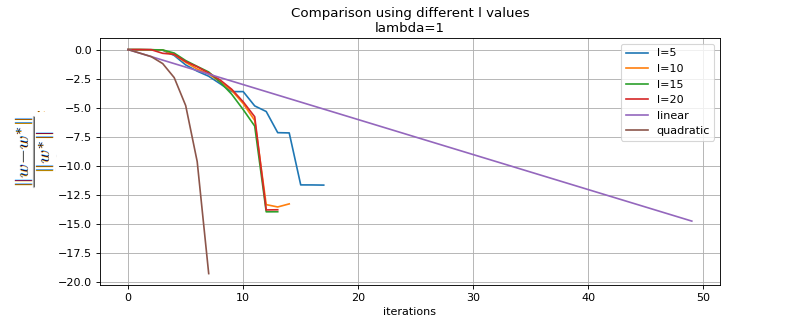
\includegraphics[width=0.8\linewidth]{images/lbfgs/lambda1.png}
    \caption{Convergence plot with $\lambda=1$ at different values of $l$}
    \label{fig:lbfgs_l_comparison}
\end{figure}

\noindent The chosen $l$ values were taken from the suggested ones by Nocedal \cite{nocedal1999numerical}, that is those inside the range $[3, 20]$ for keeping a good compromise between used memory and execution time, since we have already seen that $l$ influences the number of iterations and, therefore, the execution time of the method. We can also notice from \autoref{tab:lbfgs_results} that larger values of $l$ implies a smaller error (more evident when working with ill-conditioned matrices), this comes at no surprise since, as we already know, the more memory we use the more the Hessian is accurately approximated.
\vspace{3mm}

\noindent It's easy to notice from \autoref{fig:lbfgs_l_comparison} that for a smaller $l$ the convergence gets a little bit closer to the linear rate, meanwhile for bigger values it stays, more or less, in the middle, suggesting a super-linear convergence of the method. In our case the method was so fast that there were no relevant changes for $l>5$, since the algorithm does not reach enough iterations to show the real effect of such hyper-parameter.

\subsubsection{Analysis on \texorpdfstring{$\lambda$}{{}}} \label{subsubsec:lbfgs_lambda_analysis}
Analyzing the behavior at various values of $\lambda$ is extremely interesting and fundamental, as it explains what we will see over the plots in this subsection and in the rest of this report. The results can be briefly explained by the following observations
\begin{itemize}
    \item For larger values of $\lambda$ ($1e4$ and $1e2$) the method converges in few steps and obtains excellent results;
    \item For small $\lambda$, the algorithm requires more steps and the results get worse.
\end{itemize}

\noindent Such behavior arises when our matrix is ill-conditioned, that is when $\lambda$ is extremely small. This is caused by the fact that $\lambda$ is the smallest singular value  of $\hat{X}$ (see \ref{appendix:smallest_singular_value} and \ref{appendix:condition_number} for a better understanding) and, therefore, has a strong influence on the condition number of $\hat{X}$ making the method very unstable.

\begin{figure}[H]
    \centering
    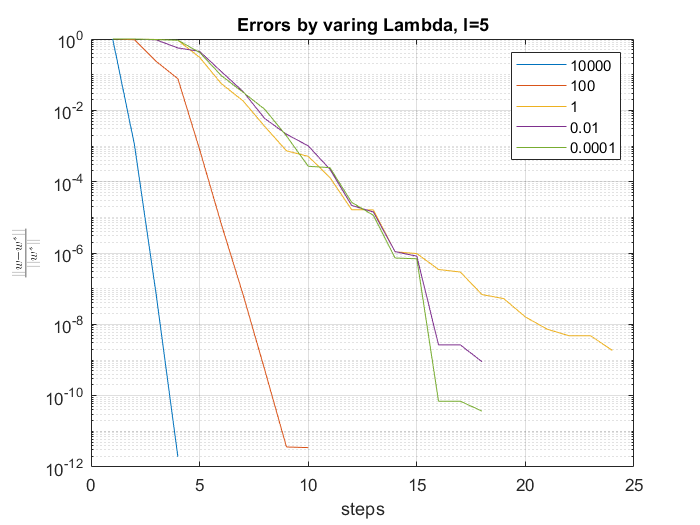
\includegraphics[width=0.8\linewidth]{images/lbfgs/errors_lambda.png}
    \caption{Errors by varying $\lambda$ with $l=5$.}
    \label{fig:lbfgs_errors_comparison_lambda}
\end{figure}

\noindent As we can see from \autoref{fig:lbfgs_errors_comparison_lambda}, the greater $\lambda$ is the better the algorithm converges even achieving a quadratic convergence rate (see \autoref{fig:lbfgs_1e4_l} for a better view) and maintaining a super-linear one for small values, confirming our previous observations and what we have stated for the convergence of L-BFGS. More plots of the L-BFGS method can be found in \ref{appendix:lbfgs_plots}.

\section{Thin QR factorization with Householder reflectors}
Inside this section we will first introduce QR factorization and Householder reflectors, then we will talk about how to solve our task with the thin variant of the former and , finally, just like we did for the L-BFGS method, we will analyze its performances.

\subsection{Overview on thin QR factorization}
For any matrix $A \in \mathbb{R}^{m\times n}$ there exist $Q \in \mathbb{R}^{m\times m}$ orthogonal and $R \in \mathbb{R}^{m\times n}$ upper triangular such that
\begin{equation}
    A=QR
    \label{eq:qr}
\end{equation}
By diving into our case, we must introduce the thin variant of \eqref{eq:qr}. Given that $\hat{X}\in \mathbb{R}^{m\times n}$, then $R$ has the following structure
\begin{center}
$\begin{bmatrix}
r_{1,1} & r_{1,2} & r_{1,3} & \dots & r_{1,n-1} & r_{1,n} \\
0 & r_{2,2} & r_{2,3} & \dots & r_{2,n-1} & r_{2,n} \\
0 & 0 & r_{3,3} & \dots & r_{3,n-1} & r_{3,n} \\
\vdots & & & & & \vdots \\
0 & 0 & 0 & \dots & r_{n-1,n-1} & r_{n-1,n} \\
0 & 0 & 0 & \dots & 0 & r_{n,n} \\
0 & 0 & 0 & \dots & 0 & 0 \\
\vdots & & & & & \vdots \\
0 & 0 & 0 & \dots & 0 & 0 \\
\end{bmatrix}$
\end{center}
Hence, $R$ can be split into two parts where the first one is $R_1\in \mathbb{R}^{n\times n}$ and, following the same reasoning, $Q$ is split into $Q_1 \in \mathbb{R}^{m\times n}$ and $Q_2 \in \mathbb{R}^{(m-n)\times n}$. Therefore, by looking at \eqref{eq:qr} and taking into account what we said just before, $\hat{X}$ can be factorized as following
\begin{equation}
    \hat{X}=QR=
    \begin{bmatrix}Q1 & Q2\end{bmatrix}\begin{bmatrix}R1 \\ 0\end{bmatrix}=Q_1 R_1
    \label{eq:qr_factorization}
\end{equation}
Before we discuss how to solve the LLS with the assigned method we need to introduce the Householder reflectors. The QR factorization, and its thin variant, can be obtained by storing the so called Householder reflectors instead of computing Q at each step, so let $x\in \mathbb{R}^n$ be any vector and let $u\in \mathbb{R}^n$ be the normalized Householder vector of $x$ such that
\begin{subequations}
    \begin{equation}
        \label{eq:householder_u}
        u=\frac{v}{\lVert v\rVert}
    \end{equation}
    where
    \begin{equation}
        \label{eq:householder_v}
        v=\begin{bmatrix}
        x_1 - \lVert x \rVert \\
        x_2 \\
        x_3 \\
        \vdots \\
        x_{n-1} \\
        x_n
        \end{bmatrix}
    \end{equation}
\label{eq:householder_vector}
\end{subequations}
\vspace{3mm}

\noindent The Householder vector defined in \eqref{eq:householder_u} is computed by algorithm\eqref{algorithm:householder_v}

\begin{algorithm}[H]
    \caption{Householder vector}
    \label{algorithm:householder_v}
    s = $\lVert x \rVert$; \\
    \If{$x(1) \geq 0$}{s=-s;}
    v = x; \\
    v(1) = v(1) - s; \\
    u = v / $\lVert v \rVert$; \\
    \Return{u, s};
\end{algorithm}

\noindent The Householder reflector of $u$ is then defined as
\begin{equation}
    H_u=I-2uu^T
    \label{eq:householder_reflector}
\end{equation}
Householder reflectors are essential for computing the QR factorization without needing to formulate Q. More formally, given a matrix $\hat{X} \in \mathbb{R}^{m \times n}$, the algorithm we have to use consists in building a list of Householder reflectors (as defined in \eqref{eq:householder_reflector}) that transform $\hat{X}$ into an un upper triangular matrix $R \in \mathbb{R}^{m \times n}$ and in storing their products as the orthogonal matrix $Q \in \mathbb{R}^{m \times m}$.

\subsection{Solving LLS with thin QR} \label{subsec:lls_qr}
Starting from \eqref{eq:qr_factorization}, we can write
\begin{equation}
\begin{aligned}
    \lVert \hat{X}w-\hat{y} \rVert &\stackrel{\footnotemark}{=} \lVert Q^T(\hat{X}w-\hat{y}) \rVert = \lVert Q^T\hat{X}w-Q^T\hat{y} \rVert = \lVert Q^TQRw-Q^T\hat{y} \rVert = \lVert Rw-Q^T\hat{y} \rVert \\
    &= \lVert \begin{bmatrix}R_1 \\ 0 \end{bmatrix}w-\begin{bmatrix}Q_1 & Q_2\end{bmatrix}^T\hat{y} \rVert = \lVert \begin{bmatrix}R_1w \\ 0 \end{bmatrix}-\begin{bmatrix}Q_1^T\hat{y} \\ Q_2^T\hat{y}\end{bmatrix}^T\rVert = \lVert \begin{bmatrix}R_1w - Q_1^T\hat{y} \\ Q_2^T\hat{y} \end{bmatrix} \rVert
\end{aligned}
\end{equation}
\footnotetext{Holds since $\lVert Qx \rVert=\lVert x \rVert$ when $Q$ is orthogonal.}

\noindent where $R_1$ and $Q_1$ are the matrices as seen in \eqref{eq:qr_factorization} and $Q_2^T\hat{y}$ is the residual of the norm, that is the optimum of our optimization problem.
\vspace{3mm}

\noindent Moreover, from the theory is known that if a matrix is factorized as in \eqref{eq:qr_factorization} and has full column rank, then the solution of LLS is given by
\begin{subequations}
    \begin{equation}
        w=R_{1}^{-1}Q_{1}^{T}\hat{y}
        \label{eq:thin_qr_solution_1}
    \end{equation}
    by stating that
    \begin{equation}
        c=Q_1^T\hat{y}
        \label{eq:thin_qr_rewrite_c}
    \end{equation}
    then \eqref{eq:thin_qr_solution_1} can be rewritten as
    \begin{equation}
        R_1w=c
        \label{eq:thin_qr_solution_2}
    \end{equation}
\label{eq:thin_qr_solution}
\end{subequations}
\vspace{3mm}

\noindent Therefore, solving the LLS problem with QR factorization is the same as solving the linear system \eqref{eq:thin_qr_solution_2}, which is an extremely easy task once $R_1$ and $Q_1$ are computed.
We now show algorithm \ref{algorithm:compute_thin_QR} that computes the thin QR factorization, without storing the Householder matrices and keeping in memory only the $m \times n$ strictly needed elements of the $Q_1$ matrix at each step. We will not show the part that solves the upper triangular system as defined by \eqref{eq:thin_qr_solution_2} since it is not relevant to the aim of this section.

\begin{algorithm}[H]
    \caption{Compute thin $QR$ factorization}
    \label{algorithm:compute_thin_QR}
    Given $A \in R^{m \times n}$\\
    $Q_{1}y = y$\\
    \For{$j = 1$ to $min(m-1,n)$}{
        $[u, s] = householder\_vector(A[j:end, j]); \triangleright$ \textbf{\autoref{algorithm:householder_v}} \\
        $A[j,j] = s;$\\
        $A[j+1:end,j] = 0;$\\
        $A[j:end,j+1:end] = A[j:end,j+1:end] - 2u*(u^T*A[j:end,j+1:end]);$\\
        $Q_{1}y[j: end] = Q_{1}y[j:end] - 2u*(u^T*Q_{1}y[j:end]);$
    }
    $R_1=A[1:n,:];$\\
    $Q_{1}y = Q_{1}y[1:n];$ \\
    \Return{$Q_{1}y, R_1$};
\end{algorithm}

\noindent As you may notice our implementation is not a strict thin qr factorization since we do not even store $Q1$, instead at each step we compute the product $Q*\hat{y}$ considering only the affected rows starting from the j-th one. Both $Q*\hat{y}$ and $R$ are computed in the main loop from \autoref{algorithm:compute_thin_QR}, keep in mind that $Q_1\hat{y}$ and $R_1$ are taken from the first n rows of $Q*\hat{y}$ and the starting matrix respectively at the end of the computation.
\vspace{3mm}

\noindent $Q*\hat{y}$ is computed as
\begin{equation}
    Q\hat{y}=H_n\dots H_1\hat{y}
    \label{eq:thin_qr_Qy}
\end{equation}

\noindent By following the definition of Householder reflector from \eqref{eq:householder_reflector}, we can see \eqref{eq:thin_qr_Qy} as
\begin{equation}
    Q\hat{y}=(I-2u_nu_n^T)\dots (I-2u_1u_1^T)\hat{y}
    \label{eq:thin_qr_Qy_reflectors}
\end{equation}

\noindent For a single iteration, \eqref{eq:thin_qr_Qy_reflectors} can be rewritten in a more easier way
\begin{equation}
    Q_i\hat{y}=(I-2u_iu_i^T)Q_i\hat{y}=Q_i\hat{y} - 2u_i(u_i^TQ_i\hat{y})
    \label{eq:thin_qr_Qy_iteration}
\end{equation}

\noindent The same reasoning can be applied to $R$
\begin{equation}
    R=H_n\dots H_1\hat{X}
    \label{eq:thin_qr_R}
\end{equation}

\noindent Without explaining again the same process seen in \eqref{eq:thin_qr_Qy_reflectors}, we can see a single iteration for computing R as
\begin{equation}
    R_i=(I-2u_iu_i^T)R_i=R_i - 2u_i(u_i^TR_i)
    \label{eq:thin_qr_R_iteration}
\end{equation}

\noindent \eqref{eq:thin_qr_Qy_iteration} and \eqref{eq:thin_qr_R_iteration} are dimensionally feasible since we operate on submatrices of $Q*y$ and $R$ as we can see from \autoref{algorithm:compute_thin_QR} (row $7$ and $8$). To give a reason on why this is more efficient, for $R$ this means doing a product between matrices of size
\begin{subequations}
    \begin{equation}
        \mathbb{R}^{(m-i)\times 1}\times (\mathbb{R}^{1\times (m-i)} \times \mathbb{R}^{(m-i)\times (n-i)})
        \label{eq:compute_R_efficient}
    \end{equation}
    instead of doing a product between two matrices of size
    \begin{equation}
        \mathbb{R}^{(m-i)\times (m-i)}\times \mathbb{R}^{(m-i)\times (n-i)}
        \label{eq:compute_R_not_efficient}
    \end{equation}
    \label{eq:compute_R}
\end{subequations}

\noindent By following \eqref{eq:compute_R_efficient} we avoid doing any product between matrices improving the execution time of our implementation, since such product requires one more order of magnitude with respect to products between vectors, hence our choice.
\vspace{3mm}

\noindent The same reasoning, of course, can be applied to $Q*\hat{y}$ where we compute products of matrices of size
\begin{equation}
    \mathbb{R}^{(m-i)\times 1}\times (\mathbb{R}^{1\times (m-i)} \times \mathbb{R}^{(m-i)\times 1})
    \label{eq:compute_Qy_efficient}
\end{equation}
    
\noindent In this way we do not need to compute $Q_1$ and then multiplying it by $\hat{y}$, instead their product is computed step by step inside the main loop of \autoref{algorithm:compute_thin_QR}.

\paragraph{Complexity}
Analyzing the computational cost of \autoref{eq:thin_qr_solution}, we notice that the vector-matrix multiplication $Q_{1}^{T}\hat{y}$ requires $\mathcal{O}(mn)$ operations, plus the time to solve the triangular system $R_1 w = Q_{1}^{T}\hat{y}$, that is $\mathcal{O}(n^2)$. Anyway, the time spent to compute this part is lower than the one required to compute the matrices $Q_1$ and $R_1$, which is $\mathcal{O}(mn^2)$.

\subsection{Backward stability}
We know aim to show the backward stability of the QR factorization (the same reasoning applies to the thin version), by first recalling the upper bound on the relative error for the LLS as we can see from \eqref{eq:upper_bound_error}
\begin{equation}
    \frac{\lVert \Tilde{w}-w \rVert}{\lVert w \rVert} \leq u
    \label{eq:upper_bound_error}
\end{equation}
where $w$ is any number and the actual solution to $\hat{X}w-\hat{y}=0$, $\Tilde{w}$ is the perturbed solution of such problem and $u$ is the so called machine precision $2^{-52}=10^{-16}$.
\vspace{3mm}

\noindent Assume that an algorithm is used to find $\hat{y}=f(w)$, we know that due to the machine precision (which is an hardware limitation) we will not get such perfect results, instead we will obtain a perturbed value $\Tilde{y}=f(\Tilde{w})$ that, in turn, will define
\begin{subequations}
    \begin{equation}
        \Delta_{\hat{y}}=\Tilde{y}-\hat{y}
        \label{eq:forward_error}
    \end{equation}
    as the forward error and
    \begin{equation}
        \Delta_w=\Tilde{w}-w
        \label{eq:backward_error}
    \end{equation}
    as the backward error.
    \label{eq:forward_backward_error}
\end{subequations}
\vspace{3mm}

\noindent Recall also that an algorithm is called backward stable if the relative backward error from \eqref{eq:backward_error} is stable, formally
\begin{equation}
    \frac{\lVert \Tilde{w}-w \rVert}{\lVert w \rVert}=\mathcal{O}(u)
    \label{eq:backward_error_stability}
\end{equation}

\noindent We first notice that doing a product with an orthogonal matrix $Q$ is backward stable, since the product $Q\circ A = Q*A+E$ (given any matrix $A^{m\times n}$) has forward error $E$ whose norm is
\begin{equation}
    \lVert E \rVert \leq \mathcal{O}(u)\lVert Q \rVert \lVert A \rVert = \mathcal{O}(u) \lVert A \rVert
    \label{eq:forward_error_norm}
\end{equation}

\noindent moreover $Q\circ A=Q(A+Q^{-1}E)$ defines the backward error $\Delta_A=Q^{-1}E$ whose norm is
\begin{equation}
    \lVert \Delta_A \rVert \leq \lVert Q^{-1} \rVert \lVert E \rVert = \mathcal{O}(u) \lVert A \rVert
    \label{eq:backward_error_norm}
\end{equation}

\noindent With \eqref{eq:forward_error_norm} and \eqref{eq:backward_error_norm} it's easy to show that the QR factorization is backward stable by perturbing $A$ with $\Delta_A$ such that $\Tilde{Q}\Tilde{R}=qr(A+\Delta_A)$. Recall that QR factorization is made up of steps as follows
\begin{equation}
    Q_k A_{k-1} = A_k
    \label{eq:qr_stability_step}
\end{equation}

\noindent considering machine precision $u$, each step starts with $\Tilde{A}_{k-1}$ (which contains even the previous errors) and produces $\Tilde{A}_k$, each single step is backward stable since the computed $\Tilde{A}_k$ and $\Tilde{u}_k$ satisfy the perturbed version of \eqref{eq:qr_stability_step}
\begin{equation}
    \Tilde{Q}_k (\Tilde{A}_{k-1}+\Delta_{k-1}) = \Tilde{A}_k
    \label{eq:qr_stability_step_perturbed}
\end{equation}

\noindent with the norm of the accumulated error at step $k-1$ as
\begin{equation}
    \lVert \Delta_{k-1} \rVert \leq \mathcal{O}(u)\lVert \Tilde{A}_{k-1} \rVert = \mathcal{O}(u) \lVert A \rVert
    \label{eq:qr_stability_error}
\end{equation}

\noindent Then, if we consider $n$ steps we can retrieve the exact result
\begin{equation}
    \Tilde{R} = A+\Delta_0+\Tilde{Q}_1^T\Delta_1+\Tilde{Q}_1^T\Tilde{Q}_2^T\Delta_2+\dots+\Tilde{Q}_1^T\Tilde{Q}_2^T\dots\Tilde{Q}_{n-1}^T\Delta_{n-1}
    \label{eq:qr_stability_exact_result}
\end{equation}

\noindent where each of the error terms is what we have seen in \eqref{eq:qr_stability_error}, by always keeping in mind that every computation is orthogonal.
\vspace{3mm}

\noindent Therefore, the QR factorization is backward stable and the computed Q and R are the exact results of $qr(A+\Delta)$ with $\lVert \Delta \rVert \leq \mathcal{O}(u) \lVert A \rVert$.
\vspace{3mm}

\noindent Moreover, while going back to our case, backward stable algorithms usually produces small residuals $r=\hat{X}w-\hat{y}$, but this does not imply that $\Tilde{w}$ is close to the actual solution $w$ as we have seen in \ref{subsec:lbfgs_analysis}. Even then is still possible to find an upper bound to such error as theorem \ref{theorem:qr_upper_bound_error} states.
\begin{theorem}
    Let $\hat{X}=Q_1R_1$ be a thin QR factorization and let $r_1=Q_1^T(\hat{X}\Tilde{w}-\hat{y})$. Then, it can be proven that $\Tilde{w}$ is the exact solution of the least square problem
    \begin{equation}
        min \lVert \hat{X}w-(\hat{y}+Q_1r_1) \rVert
        \label{eq:qr_least_square}
    \end{equation}
    thus
    \begin{equation}
        \frac{\lVert \Tilde{w}-w\rVert}{\lVert w\rVert}\leq \kappa_{rel}(LS,\hat{y})\frac{\lVert Q_1r_1\rVert}{\lVert \hat{y} \rVert}=\kappa_{rel}(LS,\hat{y})\frac{\lVert r_1\rVert}{\lVert \hat{y} \rVert}
        \label{eq:qr_upper_bound_error}
    \end{equation}
    \label{theorem:qr_upper_bound_error}
\end{theorem}
\noindent \eqref{eq:qr_upper_bound_error} states that the relative error of the LLS problem solved with thin QR factorization is bounded by the condition number relative to such problem and by the ratio between the residual and the expected values.

\subsection{Performance analysis}
We have three different purposes for the thin QR factorization algorithm:
\begin{enumerate}
    \item we have to show that our implementation scales linearly with respect to the number of rows of the input matrix.
    \item we need to check the accuracy of our implementation.
    \item we need to show the results for varying values of $\lambda$.
\end{enumerate}

\subsubsection{Linearity of thin QR with respect to the rows}\label{subsec:qr_linearity}
The project requires us to implement a thin QR factorization algorithm that scales linearly with respect to the biggest dimension of the number of rows of a matrix, in order to prove this behavior, we created 20 $m \times n$ random matrices, with $n$ fixed and equal to 200, whereas $m$ spaces from 1000 to 5750 with a step size equal to 250. For each configuration, we ran our thin QR factorization algorithm 10 times, measuring the average completion time and then we plotted the results as shown in \autoref{fig:avg_time_qr}.
\begin{figure}[H]
    \centering
    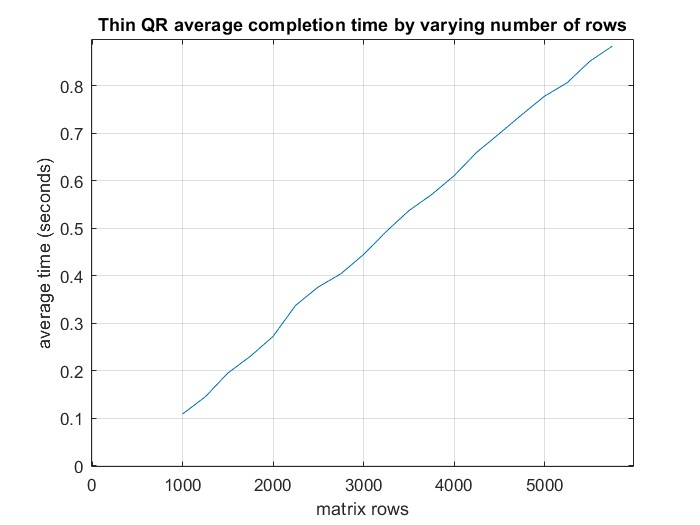
\includegraphics[width = 0.8\linewidth]{images/thin_qr/avg_time_qr.jpg}
    \caption{Thin QR average completion time by varying number of rows.}
    \label{fig:avg_time_qr}
\end{figure}

\noindent As \autoref{fig:avg_time_qr} shows, our implementation of thin QR scales linearly with the number of rows which is expected as we know that its complexity is $\mathcal{O}(mn^2)$ from the last paragraph of \ref{subsec:lls_qr}.

\subsubsection{Accuracy of thin QR}
We are also interested in the accuracy of our thin QR implementation to know how it factorizes our matrix $\hat{X}$ when $\kappa(\hat{X})$ becomes high (we already know this is caused by $\lambda$ as talked in \ref{appendix:condition_number}), such metric is defined as
\begin{equation}
    \frac{\lVert \hat{X} - Q_1R_1\rVert}{\lVert \hat{X}\rVert}
    \label{eq:thin_qr_accuracy}
\end{equation}
where $Q_1$ and $R_1$ are the matrices obtained by our thin qr factorization.
\vspace{3mm}

\noindent In short, we want to know how accurately our thin QR rebuilds the starting matrix. For such purpose, \autoref{tab:thin_qr_accuracy} shows the accuracies achieved by our method compared to the ones from the matlab implementation (called "economical thin QR") and the distance between them.
\begin{table}[H]
\centering
\begin{tabular}{c|c|c|c} \hline \hline
    $\lambda$ & Our accuracy & Matlab accuracy & $\Delta$ accuracies\\
    \hline \hline
    
    \rowcolor{gray!30} $10^4$ & $1.865168 \times 10^{-15}$ & $3.088531 \times 10^{-15}$ & $1.223363 \times 10^{-15}$ \\
    
    $10^2$ & $9.94962 \times 10^{-16}$ & $1.602198 \times 10^{-15}$ & $6.072354 \times 10^{-16}$ \\
    
    \rowcolor{gray!30} $1$ & $7.463726 \times 10^{-16}$ & $7.450506 \times 10^{-16}$ & $1.321951 \times 10^{-18}$ \\
    
    $10^{-2}$ & $7.908642 \times 10^{-16}$ & $7.630684 \times 10^{-16}$ & $2.779588 \times 10^{-17}$ \\
    
    \rowcolor{gray!30} $10^{-4}$ & $7.542911 \times 10^{-16}$ & $7.424282 \times 10^{-16}$ & $1.186286 \times 10^{-17}$ \\
    \hline \hline
\end{tabular}
\caption{Thin QR accuracy.}
\label{tab:thin_qr_accuracy}
\end{table}

\noindent From \autoref{tab:thin_qr_accuracy} we can see that our accuracy is close to $\mathcal{O}(u)=1e-16$ meaning that our implementations is, indeed, correct, as expected from a backward stable algorithm. Moreover our accuracy is extremely close to the one achieved by matlab, giving us a nice confidence boost for the next steps in this performance analysis.

\subsubsection{Results}
Since the only hyper-parameter for the thin QR is $\lambda$ we will show how the results change when the latter assumes different values, moreover we will not show the standard deviation for each configuration since it's very close to $0$ given the fact that thin QR is not iterative.
\vspace{3mm}

\noindent The considered values for $\lambda$ are the same seen in \ref{subsec:lbfgs_analysis}, but this time we consider one more metric which is the gradient of the function $\nabla f(w)$ in $w$, since we did not use it as stop condition. As for the L-BFGS, using the relative error on $w$ is fine given the fact that $w^*$ is unique, thanks to what we have seen in \ref{subsec:introduction_convexity}.
\vspace{3mm}

\noindent We also consider the upper bound from \eqref{eq:qr_upper_bound_error} since it gives us a nice information about the maximum relative error we can achieve by computing the solution using non-exact arithmetic. Moreover, \eqref{eq:qr_upper_bound_error} can be rewritten as 
\begin{equation}
    \frac{\lVert w - w^* \lVert}{\lVert w^*\rVert}\leq\kappa_{rel}(LS,\hat{y})\frac{\lVert r_1\rVert}{\lVert \hat{y} \rVert}\stackrel{\footnotemark}{=} \frac{\kappa(\hat{X})}{\lVert \hat{X}w \rVert}\lVert r_1 \rVert
    \label{eq:qr_upper_bound_performance}
\end{equation}
\footnotetext{recall that $\kappa_{rel}(LS,\hat{y})=\frac{\kappa(\hat{X})}{\cos{\theta}}$, where $\cos{\theta}=\frac{\lVert \hat{X}w \rVert}{\lVert \hat{y} \rVert}$.}

\noindent We can now show the results achieved by our implementation in \autoref{tab:thin_qr_results} before doing a brief explanation about them.
\begin{table}[H]
\centering
\begin{tabular}{c|c|c|c|c} \hline \hline
    $\lambda$ & $\frac{\lVert w - w^* \lVert}{\lVert w^*\rVert}$ & $\frac{\lVert \hat{X}w - \hat{y}\rVert }{\lVert \hat{y} \rVert}$ & $\lVert \nabla f(w) \rVert$ & $\frac{\kappa(\hat{X})}{\lVert \hat{X}w \rVert}\lVert r_1 \rVert$ \eqref{eq:qr_upper_bound_performance} \\ \hline \hline
    
    \rowcolor{gray!30} $10^4$ & $7.3825 \times 10^{-14}$ & $9.9959 \times 10^{-1}$& $1.8069 \times 10^{-10}$ & $1.0512 \times 10^{-13}$ \\
    
    $10^2$ & $1.5650\times 10^{-14}$ & $9.1160 \times 10^{-1}$ & $6.0329 \times 10^{-12}$ & $2.7837\times 10^{-14}$ \\
    
    \rowcolor{gray!30} $1$ & $2.0354 \times 10^{-14}$ & $5.3405 \times 10^{-2}$ & $2.7046 \times 10^{-12}$ & $1.1681\times 10^{-12}$ \\
    
    $10^{-2}$ & $9.0120 \times 10^{-14}$ & $5.4414 \times 10^{-4}$ & $4.6584 \times 10^{-12}$ & $2.0006\times 10^{-10}$ \\
    
    \rowcolor{gray!30} $10^{-4}$ & $8.1724 \times 10^{-14}$ & $5.4071 \times 10^{-6}$ & $6.1100 \times 10^{-12}$ & $1.0513\times 10^{-8}$ \\
    \hline \hline
\end{tabular}
\caption{Thin QR results. $w^{*}$ is the Matlab solution from $\hat{X} \backslash\hat{y}$.}
\label{tab:thin_qr_results}
\end{table}

\noindent The execution time is more or less $9.8s$ for each configuration so we decided not to report it. By considering the upper bound from \eqref{eq:qr_upper_bound_performance}, we can notice how it decreases as $\lambda$ increases since $\kappa(\hat{X})$ starts to get bigger and bigger. Anyway, the bound always holds for our implementation, even for small values of $\lambda$, as we expected from the theory.
\vspace{3mm}

\noindent Furthermore, we noticed that the residuals follow the same behavior as we have seen for the L-BFGS in \ref{subsec:lbfgs_analysis}, that is the decreasing of the relative residual as the value of $\lambda$ decreases.

\section{Conjugate gradient}\label{sec:conjugate_gradient}
In this section we will talk about the conjugate gradient method in the same way we did for L-BFGS and thin QR, by first introducing the algorithm itself and then by analyzing its complexity and the performances obtained by applying to our case. 

\subsection{Overview on conjugate gradient}
The conjugate gradient is an iterative algorithm for solving linear systems of equations
\begin{equation}
    Ax=b
    \label{eq:cg_linear_system}
\end{equation}
where $A \in \mathbb{R}^{n\times n}$ is a symmetric positive definite matrix \footnote{$X=X^T$ and $zAz^T>0$ $\forall z \neq 0 \in \mathbb{R}^{n}$} and $x,b \in \mathbb{R}^{n}$, where $x$ is called as the unique solution. Since $A$ is symmetric positive definite, then \eqref{eq:cg_linear_system} can be stated as a minimization problem (a strictly convex one to be more precise)
\begin{subequations}
    \begin{equation}
        min\hspace{1mm} \phi(x) \stackrel{def}{=} \frac{1}{2}x^TAx - b^Tx
        \label{eq:cg_minimization_function}
    \end{equation}
    \begin{equation}
        \nabla \phi(x) = Ax-b \stackrel{def}{=} r(x)
        \label{eq:cg_minimization_gradient}
    \end{equation}
    \label{eq:cg_minimization}
\end{subequations}

\noindent In short, minimizing \eqref{eq:cg_minimization_function} means that we need to solve either \eqref{eq:cg_minimization_gradient} (with $r(x)=0$) or \eqref{eq:cg_linear_system}.

\subsubsection{Conjugate direction methods}
\noindent As the name suggests the conjugate gradient method exploits a property called \textit{conjugacy} to generate a set of vectors. A set of non-zero vectors $\{ p_0, p_1 \dots p_l\}$ is known as \textit{conjugate} of a symmetric definite positive matrix $A$ if
\begin{equation}
    p_i^TAp_j=0, \hspace{3mm} \forall i\neq j
    \label{eq:cg_conjugacy}
\end{equation}

\noindent \eqref{eq:cg_conjugacy} is vital to minimize \eqref{eq:cg_minimization_function} in, at maximum, $n$ steps, but first we need to consider the \textit{conjugate direction} method. Given a starting point $x_0 \in \mathbb{R}^n$ and a set of conjugate directions $\{ p_0, p_1 \dots p_{n-1}\}$, the sequence $\{ x_k\}$ is generated step by step by
\begin{equation}
    x_{k+1} = x_k + \alpha_kp_k
    \label{eq:cg_step}
\end{equation}

\noindent \eqref{eq:cg_step} seems identical to what we have seen for the L-BFGS in \eqref{eq:bfgs_step} and also the step size $\alpha$ will be similar, which is now defined as
\begin{equation}
    \alpha_k = -\frac{r_k^Tp_k}{p_k^TAp_k}
    \label{eq:cg_alpha}
\end{equation}

\noindent We now have enough tools for theorem \ref{theorem:cg_conjugate_direction} (theorem 5.1 from \cite{nocedal1999numerical}, the proof can also be found there).
\begin{theorem}
    For any $x_0 \in \mathbb{R}^n$ the sequence $\{ x_k\}$ generated by the conjugate direction algorithm \eqref{eq:cg_step}, then \eqref{eq:cg_alpha} converges to the solution $x^*$ of the linear system \eqref{eq:cg_linear_system} in at most $n$ steps.
    \label{theorem:cg_conjugate_direction}
\end{theorem}

\noindent Theorem \ref{theorem:cg_conjugate_direction} tell us some properties of conjugate directions:
\begin{enumerate}
    \item If $A$ is diagonal, then the contours of \eqref{eq:cg_minimization_function} are ellipses whose axes are aligned with the coordinate directions, therefore, we can find the minimum by performing one-dimensional minimizations along the coordinate directions $e_1, e_2, \dots e_n$. If $A$ is not diagonal we need to precondition it in order to obtain the same behaviour.
    \item When the Hessian is diagonal, each coordinate minimization determines one of the components of the solution $x^*$.
\end{enumerate}

\noindent The second property holds even when the Hessian is not diagonal and this is proven by theorem \ref{theorem:expanding_subspace_minimization} (theorem 5.2 and proof from \cite{nocedal1999numerical}).
\begin{theorem}
    Let $x_0 \in \mathbb{R}^n$ be any starting point and suppose that the sequence $\{ xk \}$ is generated by the conjugate direction algorithm \eqref{eq:cg_step}, \eqref{eq:cg_alpha}. Then
    \begin{equation}
        r_k^Tp_i = 0 \hspace{3mm} for \hspace{1mm} i=0,...k-1
        \label{eq:cg_residual_direction}
    \end{equation}
    and $x_k$ is the minimizer of \eqref{eq:cg_minimization_function} over the set
    \begin{equation}
        \{x | x = x_0 +span\{ p_0, p_1,\dots, p_{k-1}\} \}
    \end{equation}
    \label{theorem:expanding_subspace_minimization}
\end{theorem}

\subsubsection{Conjugate gradient method}
As the name suggest, the conjugate gradient method is a conjugate direction method with the very nice fact that to compute a new vector $p_k$ based only on $p_{k-1}$, hence it does not need the entire conjugate set. This implies that the method requires little storage and computations.
\vspace{3mm}

\noindent In the conjugate gradient method, each direction $p_k$ is chosen to be a linear combination of the negative residual $-rk$ (which, by \eqref{eq:cg_minimization_gradient} is the steepest direction for \eqref{eq:cg_minimization_function}) and the previous direction $p_{k-1}$, formally
\begin{equation}
    p_k = -r_k + \beta_kp_{k-1}
    \label{eq:cg_direction}
\end{equation}

\noindent where $\beta_k$ is a value determined by the requirement that $p_k$ and $p_{k_1}$ must be conjugate with respect to $A$, moreover, by doing the product of \eqref{eq:cg_direction} with $p^T_{k-1}A$ and imposing the condition that $p^T_{k-1}Ap_k=0$, we find that
\begin{equation}
    \beta_k = \frac{r^T_kAp_{k-1}}{p^T_{k-1}Ap_{k-1}}
    \label{eq:cg_beta}
\end{equation}

\noindent We need to show that the directions $p_0, p_1,\dots, p_{n-1}$ are indeed conjugate, which by theorem \ref{theorem:cg_conjugate_direction} implies that the method terminates in $n$ steps. Theorem \ref{theorem:cg_krylov} (theorem 5.3 from \cite{nocedal1999numerical}) establishes this property and two other important properties:
\begin{enumerate}
    \item The residuals $r_i$ are mutually orthogonal.
    \item Each search direction $p_k$ and residual $r_k$ is contained in the \textit{Krylov subspace of degree $k$ for $r_0$}, defined as
    \begin{equation}
        K(r_0, k) \stackrel{def}{\approx} span\{ r_0, Ar_0, \dots, A^kr_0 \}
        \label{eq:cg_krylov_subspace}
    \end{equation}
\end{enumerate}

\begin{theorem}
Suppose that the k-th iterate generated by the conjugate gradient method is not the solution point $x^*$. The following four properties hold
    \begin{subequations}
        \begin{equation}
            r_k^Tr_i = 0, \hspace{3mm} for\hspace{1mm} i=0,\dots, k-1
        \end{equation}
        \begin{equation}
            span\{ r_0,r_1,\dots,r_k \} = span\{ r_0, Ar_0,\dots, A^kr_0\}
        \end{equation}
        \begin{equation}
            span\{ p_0,p_1,\dots,p_k \} = span\{ r_0, Ar_0,\dots, A^kr_0\}
            \label{eq:cg_krylov_property}
        \end{equation}
        \begin{equation}
            p^T_kAp_i = 0, \hspace{3mm} for\hspace{1mm} i=0, \dots, k-1
        \end{equation}
    \end{subequations}
    \label{theorem:cg_krylov}
\end{theorem}

\noindent The proof of theorem \ref{theorem:cg_krylov} can be found after theorem 5.3 from \cite{nocedal1999numerical}. As last thing for this part, we can rewrite \eqref{eq:cg_alpha} by using \eqref{eq:cg_direction} and \eqref{eq:cg_residual_direction} to obtain
\begin{equation}
    \alpha_k = -\frac{r_k^Tp_k}{p_k^TAp_k} = -\frac{r_k^T(-r_k+\beta_kp_{k-1})}{p_k^TAp_k} = \frac{r_k^Tr_k}{p_k^TAp_k}
    \label{eq:cg_alpha_efficient}
\end{equation}

\noindent Moreover, noting the relation between \eqref{eq:cg_step}, and the k-th residual $r_k=Ax_k-b$, we can write
\begin{equation}
    r_{k+1} = rk+\alpha_kAp_k
    \label{eq:cg_residual}
\end{equation}

\noindent We can also rewrite \eqref{eq:cg_beta} based, again, on \eqref{eq:cg_direction}, \eqref{eq:cg_residual_direction} and \eqref{eq:cg_residual}
\begin{equation}
    \beta_k = \frac{r^T_kAp_{k-1}}{p^T_{k-1}Ap_{k-1}} = \frac{r^T_k\frac{r_k-r_{k-1}}{\alpha_{k-1}}}{p^T_{k-1}\frac{r_k-r_{k-1}}{\alpha_{k-1}}} = \frac{r^T_k(r_k-r_{k-1})}{p^T_{k-1}(r_k-r_{k-1})} = -\frac{r^T_kr_k}{r^T_{k-1}p_{k-1}} = \frac{r^T_kr_k}{r^T_{k-1}r_{k-1}}
    \label{eq:cg_beta_efficient}
\end{equation}

\noindent We now have everything needed to build the conjugate gradient algorithm and to apply to our case.

\subsection{Solving LLS with conjugate gradient}\label{subsec:solve_LLS_cg}
Diving into our lls problem we first notice that $\hat{X}$ is not symmetric positive definite, hence we can not apply the conjugate gradient method in a straightforward way. But, as we have seen in \ref{subsec:introduction_lls}, the solution to the lls problem is obtained by solving \eqref{eq:normal_equation} and, luckily for us, $\hat{X}^T\hat{X}$ is symmetric positive definite (this is also the Hessian of the lls which we have shown to be positive definite in \ref{subsec:introduction_convexity}), so we can apply that to our case.
\vspace{3mm}

\noindent The optimal solution $w_*$, therefore, can be found in the following way
\begin{equation}
    w^T_*\hat{X}^T\hat{X}=\hat{y}^T\hat{X} \Longleftrightarrow \hat{X}^T\hat{X}w_*=\hat{X}^T\hat{y}
    \label{eq:cg_solving_normal_equation}
\end{equation}

\noindent $\hat{X}^T\hat{X} \in \mathbb{R}^{n \times n}$ has full column rank, therefore is symmetric positive definite and we can now solve the lls with the conjugate gradient, but, before we proceed further, we should rewrite \eqref{eq:cg_solving_normal_equation} in a more readable way
\begin{equation}
    \hat{X}^T\hat{X}w_*=\hat{X}^T\hat{y} \Longleftrightarrow Aw_*=b
    \label{eq:cg_normal_equation_rewritten}
\end{equation}

\noindent From now on we will refer to the right side of \eqref{eq:cg_normal_equation_rewritten} over the next sections. We now have everything needed to show the conjugate gradient method in \autoref{algorithm:cg}

\begin{algorithm}[H]
    \caption{Conjugate gradient}
    \label{algorithm:cg}
    Given $x_0 \in R^m$;\\
    $r_0=Ax_0-b$;\\
    $p_0=-r_0$;\\
    $k=0$;\\
    \While{$r_k\neq 0$} {
        $\alpha_k =  \frac{r_k^Tr_k}{p_k^TAp_k}$;\\
        $x_{k+1} = x_k + \alpha_kp_k$;\\
        $r_{k+1} = r_k + \alpha_kAp_k$;\\
        $\beta_{k+1} = \frac{r^T_{k+1}r_{k+1}}{r^T_kr_k}$;\\
        $p_{k+1}=-r_{k+1}+\beta_{k+1}p_k$;\\
        $k=k+1$;\\
    }
    \Return{$x_{k+1}$};
\end{algorithm}

\noindent Of course, we can improve \autoref{algorithm:cg} by computing $Ap_k$, $r^T_kr_k$ before $\alpha_k$ and $\beta_{k+1}$ in order to obtain a better execution time.
\vspace{3mm}

\noindent Moreover, in order to apply the conjugate gradient algorithm to solve the lls problem, we need to compute the matrix product $A = \hat{X^T}\hat{X}$, as we can see from \eqref{eq:cg_normal_equation_rewritten}. Therefore, the resulting matrix has a conditioning number $\kappa(A) = \kappa(\hat{X})^2$ and this implies that $A$ is extremely ill-conditioned when $\lambda$ is small (recall the conditioning number of our matrices $\hat{X}$ from \autoref{tab:condition_number}). This issue can be mitigated by avoiding to form the matrix $A$ explicitly, because it is less sparse than $\hat{X}$.
\vspace{3mm}

\noindent By looking at \autoref{algorithm:cg}, we can compute $r_0$ by first finding the product $\hat{X}x_{0}$, and then $\hat{X^T}\hat{X}x_{0}$. Also, the update of $\alpha_k$ should be modified as following
\begin{equation}
    \alpha_k =  \frac{r_k^Tr_k}{(\hat{X}p_k)^{T}\hat{X}p_k}
    \label{eq:cg_rewritten_alpha}
\end{equation}
knowing that the inner product $\langle p, \hat{X}^T \hat{X} p \rangle = \langle \hat{X}p, \hat{X}p \rangle$.
\vspace{3mm}

\noindent Finally, we modify the update of $r_k$ with
\begin{equation}
    r_{k+1} = r_k + \alpha_k \hat{X}^T (\hat{X} p_k)
\end{equation}
This normal equations approach was suggested by Björck and Elfving \cite{bjorck1979accelerated}, and it allowed us to reach a solution that is an order of magnitude better than our original approach.

\subsection{Convergence and complexity}
From \autoref{theorem:cg_conjugate_direction} we know that conjugate gradient converges at the solution in at most $n$ steps, this can be improved when the distribution of the eigenvalues of $A$ has certain features. First, we can notice that at each step of the conjugate gradient method, the error term $e_{k+1}=w_{k+1}-w^*$ can be rewritten as
\begin{equation}
    e_{k+1} = e_0 + span\{r_0,Ar_0,A^2r_0,\dots,A^kr_0\} = e_0 + span\{Ae_0,A^2e_0,\dots,A^ke_0\}
    \label{eq:cg_error_subspace}
\end{equation}
then by considering a polynomial $P_k(A)$ of degree $k$, we can state that the error term assumes the following form
\begin{equation}
    e_{k+1} = w_{k+1}-w^* = P_k(A)(w_0-w^*) = P_k(A)e_0 = \left( I+\sum_{i=1}^k \gamma_iA^i \right)e_0
    \label{eq:cg_wk+1_and_wstar}
\end{equation}
for some constants $\gamma_i$ related to $\beta_i$ and $\alpha_i$ (this fact is not important for the pursuance of this section). What is interesting to us is the fact that the algorithm chooses each $\gamma_i$ in order to minimize
\begin{equation}
    \lVert e_{k+1}\rVert_A^2 = e_{k+1}^TAe_{k+1} = (w_{k+1}-w^*)^TA(w_{k+1}-w^*)
    \label{eq:cg_weighted_norm_c}
\end{equation}

\noindent Moving now forward on our analysis, let $0<\theta_1\leq\dots\leq\theta_m$ be the eigenvalues of $A$ and let $v_1,\dots, v_n$ be the corresponding orthonormal eigenvectors, such that
\begin{equation}
    A=\sum^m_{i=1}\theta_iv_iv^T_i
    \label{eq:cg_rewritten_matrix}
\end{equation}
then, we can rewrite $e_0$ as
\begin{equation}
    e_0=w_0-w^*=\sum_{i=1}^n\xi_i v_i
    \label{eq:cg_w0_wstar}
\end{equation}
for some coefficient $\xi_i$. Moreover, $P_k$ can take either a scalar or a matrix as argument and the results will be the same, so it can be shown that
\begin{equation}
    P_k(A)v_i=P_k(\theta_i)v_i \hspace{3mm} \forall i=1,\dots,m
\end{equation}

\noindent Therefore, by plugging \eqref{eq:cg_w0_wstar} into \eqref{eq:cg_wk+1_and_wstar} we obtain that
\begin{equation}
    e_{k+1}=w_{k+1}-w^*=\sum_{i=1}^n\xi_i P_k(\theta_i)v_i
    \label{eq:cg_rewritten_xk+1_and_xstar}
\end{equation}

\noindent By looking at \eqref{eq:cg_weighted_norm_c}, we can also rewrite \eqref{eq:cg_rewritten_xk+1_and_xstar} as
\begin{equation}
    \lVert e_{k+1}\rVert_A^2=\lVert w_{k+1}-w^*\rVert^2_A=\sum_{i=1}^n\xi_i^2[P_k(\theta_i)]^2\theta_i
\end{equation}

\noindent Then, by extracting the largest of the terms $[P_k(\theta_i)]^2$ we retrieve that
\begin{equation}
     \lVert w_{k+1}-w^*\rVert^2_A\leq \min_{P_k} \max_{1\leq i\leq n}[P_k(\theta_i)]^2(\sum_{j}^n\theta_j\xi^2_j)=\min_{P_k} \max_{1\leq i\leq n}[P_k(\theta_i)]^2\lVert w_0-w^*\rVert_A^2
     \label{eq:cg_upper_bound}
\end{equation}

\noindent \eqref{eq:cg_upper_bound} gives us an upper bound, allowing us to estimate the convergence rate of the method by estimating
\begin{equation}
    \min_{P_k} \max_{1\leq i\leq n}[P_k(\theta_i)]^2
    \label{eq:cg_upper_bound_quantity}
\end{equation}
In short, we need to look for a $P_k$ that minimizes \eqref{eq:cg_upper_bound_quantity}.
\vspace{3mm}

\noindent Following what we have seen in this section until now, we can introduce \autoref{theorem:cg_eigenvalues} and Theorem \ref{theorem:cg_eigenvalues_estimate} (theorems 5.4 and 5.5 from \cite{nocedal1999numerical}, their proofs are also there).
\begin{theorem}
    If A has only $r$ distinct eigenvalues, then the CG iteration will terminate at the solution in at most $r$ iterations.
    \label{theorem:cg_eigenvalues}
\end{theorem}
Following the same reasoning, Leunberger derived an estimate
\begin{theorem}
    If $A$ has eigenvalues $\theta_1\leq\dots\leq\theta_n$, we have that
    \begin{equation}
        \lVert w_{k+1}-w^*\rVert_A^2\leq \left(\frac{\theta_{n-k}-\theta_1}{\theta_{n-k}+\theta_1}\right)^2\lVert w_0-w^*\rVert_A^2
    \end{equation}
    \label{theorem:cg_eigenvalues_estimate}
\end{theorem}
By defining $\epsilon=\theta_{n-j}-\theta_1$, Theorem \ref{theorem:cg_eigenvalues_estimate} tells us that after $j+1$ steps of applying the method, we obtain
\begin{equation}
    \lVert e_j\rVert_A\approx\epsilon\lVert e_0\rVert_A
    \label{eq:cg_epsilon}
\end{equation}
Another last thing is the fact that $\epsilon$ from \eqref{eq:cg_epsilon} can be rewritten in terms of $\kappa(A)=\frac{\theta_m}{\theta_1}$, giving us the following
\begin{equation}
    \lVert e_j \rVert_A=\lVert w_{j}-w^*\rVert_A\approx2\left(\frac{\sqrt{\kappa(A)}-1}{\sqrt{\kappa(A)}+1}\right)^j\lVert e_0\rVert_A
    \label{eq:cg_rewritten_epsilon}
\end{equation}
The bound from \eqref{eq:cg_rewritten_epsilon} is a large overestimation of the error, but it could be useful when the only information we know about $A$ are its maximum and minimum eigenvalues.

\paragraph{Complexity}
The most expensive operations inside the conjugate gradient algorithm are the matrix-vector products that, in general, require $\mathcal{O}(z)$ operations, where $z$ is the number of non-zero entries of the matrix. If the matrix $A \in \mathbb{R}^{n \times n}$ is sparse, then $z \in \mathcal{O}(n)$. This holds also for our case, in fact the $\hat{X}$ matrix is sparse and almost square: the non-zeros entries are only in the diagonal of $\lambda I$ and in the first 12 rows as we can see from \autoref{fig:sparsity_x_hat}.
\begin{figure}[H]
    \centering
    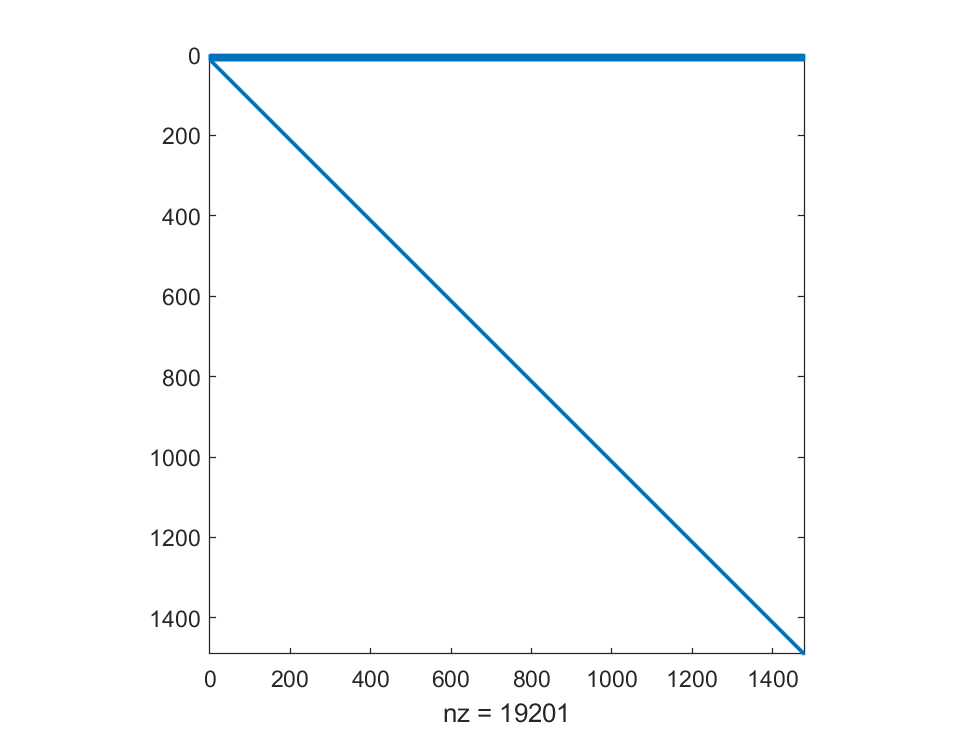
\includegraphics[width = 0.8\linewidth]{images/cg/spy_Xhat.png}
    \caption{Sparsity of $\hat{X}$, $nz$ is the number of non-zero entries.}
    \label{fig:sparsity_x_hat}
\end{figure}

\noindent Now, suppose we wish to perform enough iterations to reduce the norm of the error by a factor of $\epsilon$, that is $\lVert w_{i}-w^*\rVert_A \leq \epsilon \lVert w_{i}-w^*\rVert_A $, then \eqref{eq:cg_rewritten_epsilon} comes at our help suggesting that the maximum number of iterations required from this algorithm is
\begin{equation}
    i \leq \ceil*{\frac{1}{2} \sqrt{\kappa} \log{\left(\frac{2}{\epsilon}\right)}}
    \label{eq:cg_maximum_iterations}
\end{equation}
and we can conclude that the conjugate gradient has a time complexity of $\mathcal{O}(z\sqrt{\kappa})$. This analysis was inspired by the one from Shewchuk et al. \cite{shewchuk1994introduction}.

\subsection{Performance analysis} \label{subsec:cg_performance}

In this section we will take into account the condition number of the matrix $\hat{X}$ rather than the one of $A = \hat{X}^T \hat{X}$ because the CG algorithm \eqref{algorithm:cg} does not explicitly compute it.

\subsubsection{Empirical observation on the execution time}
We know that the algorithm runs in $\mathcal{O}(z\sqrt{\kappa(\hat{X})})$, so we might expect a linear behavior till $\sqrt{\kappa(\hat{X})} < z$. From this point on, the complexity only depends on $\sqrt{\kappa(\hat{X})}$. Unfortunately, this quantity grows exponentially and this implies that when it exceeds the amount of non-zero values of $\hat{X}$, the execution time of the algorithm starts to grow exponentially, as shown in \autoref{fig:cg_plot_conditioning}.

\begin{figure}[H]
    \centering
    \subfloat[Condition number of $\hat{X}$ by varying $\lambda$.]{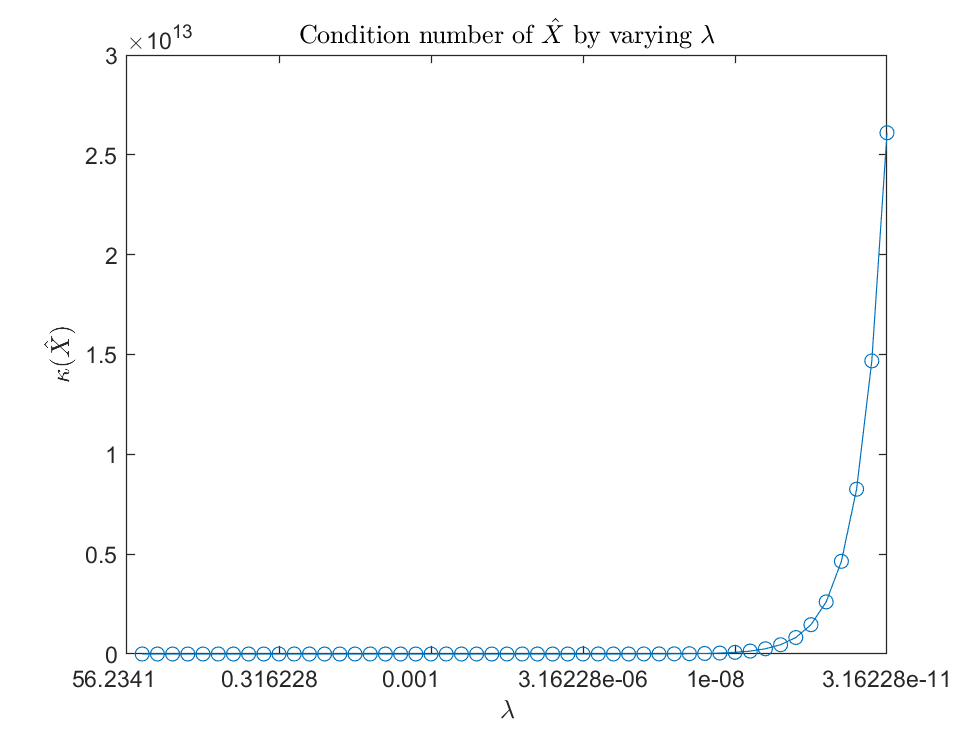
\includegraphics[width=0.62\linewidth]{images/cg/condition_number_X_hat.png}} \\
    \subfloat[Execution time of CG algorithm by varying $\kappa(\hat{X})$.]{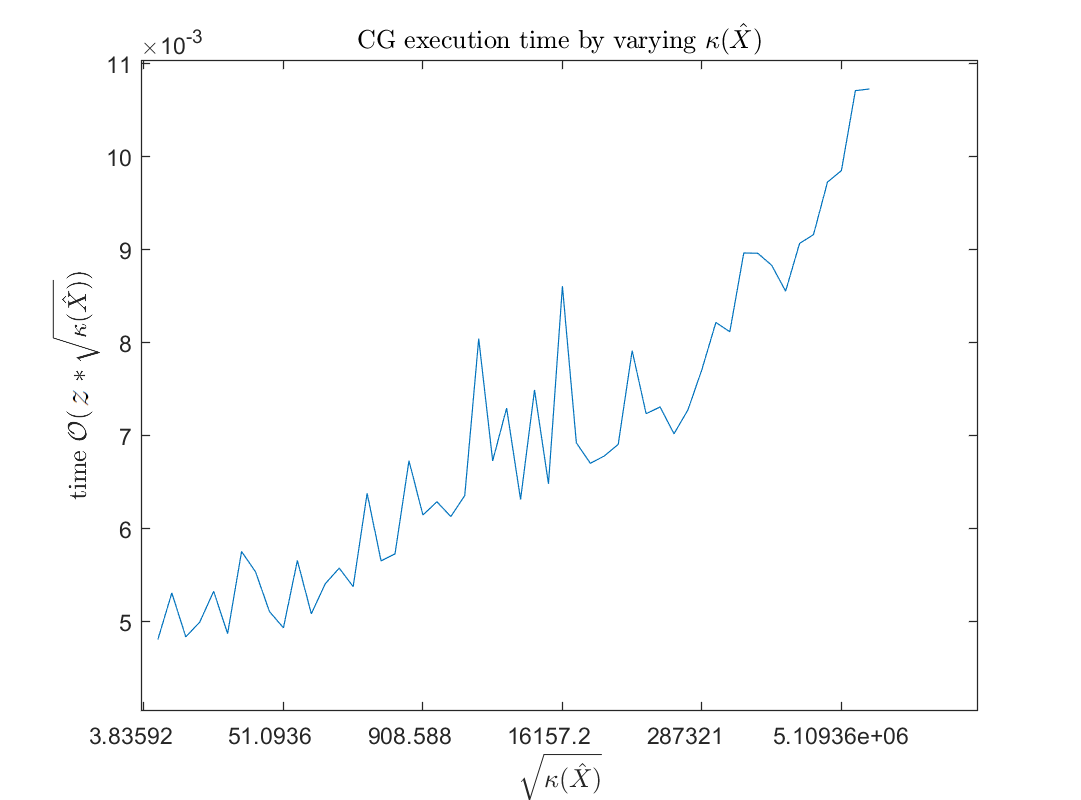
\includegraphics[width=0.62\linewidth]{images/cg/exec_time_cg_cond.png}}
    \caption{Side by side comparison between $\kappa(\hat{X})$ and the execution time of the CG algorithm.}
    \label{fig:cg_plot_conditioning}
\end{figure}

\subsubsection{Superlinear convergence ratio}
By plotting the relative errors $\frac{\lVert w-w^*\rVert}{\lVert w^*\rVert}$ we observed that the conjugate gradient algorithm has a super-linear convergence ratio, this is also confirmed by Beckermann et al. \cite{beckermann2001superlinear}. We decided to show how the conjugate gradient convergence rate changes as $\lambda$ assumes different values, just as we did for the others methods.
\begin{figure}[H]
    \centering
    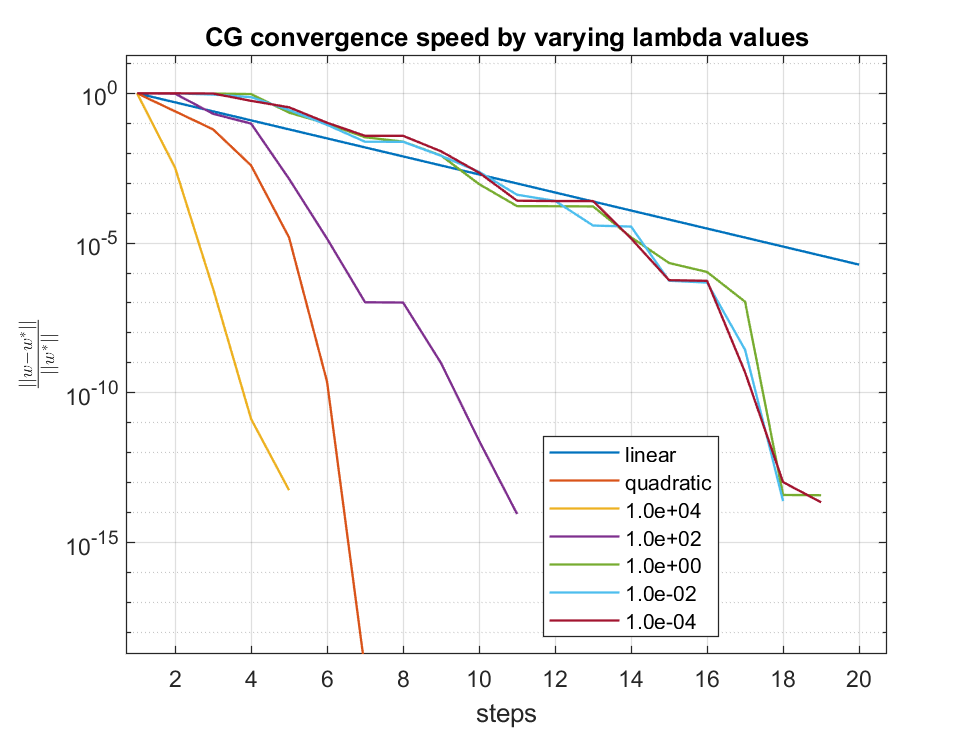
\includegraphics[width = 0.8\linewidth]{images/cg/superlinear_cg.png}
    \caption{CG convergence speed by varying lambdas values.}
    \label{fig:superlinear_cg}
\end{figure}

\noindent As we can see from \autoref{fig:superlinear_cg}, the method reaches a worse convergence ratio as $\lambda$ decreases, like we have seen for L-BFGS.

\subsubsection{Results}
The number of the distinct eigenvalues of $A = \hat{X}^{T} \hat{X}$ is 13, as stated in \ref{appendix:eigenvalues_singular_values}, so we expect to find a solution at most in 13 steps if we were in exact arithmetic as stated by \autoref{theorem:cg_eigenvalues}. As shown in \autoref{tab:cg_results}, CG algorithm found a solution requiring a less number of steps with respect to the theoretical maximum until the matrix $\hat{X}$ is well-conditioned. When $\kappa(\hat{X})$ increases, the algorithm took some more steps to converge. Furthermore, by storing the matrix $\hat{X}$ as sparse, the algorithm runs two order of magnitude faster, doing the same number of iterations. The solution has a relative error of $10^{-14}$ with respect to the Matlab solution $w^* = \hat{X}\backslash \hat{y}$, moreover, we need to point out, again, that using the relative error on $w$ is doable since $w^*$ is unique.
\begin{table}[H]
\centering
\begin{tabular}{c|c|c|c|c} \hline \hline
    $\lambda$&$\frac{\lVert w - w^{*} \lVert}{\rVert w^{*} \lVert}$ & $\frac{\lVert \hat{X}w - \hat{y} \lVert }{\lVert \hat{y} \lVert}$ & steps & time (sec)\\ \hline \hline
    
    \rowcolor{gray!30} $10^4$ & $(2.768 \pm 2.726)\times 10^{-14}$ & $ 9.996 \times 10^{-1} \pm 3.268 \times 10^{-4}$ & $4$& $5.5 \times 10^{-4}$\\
    
    $10^2$ & $ 1.477 \times 10^{-14} \pm 5.881 \times 10^{-15}$ & $ 9.336 \times 10^{-1} \pm 4.214 \times 10^{-2}$ & $10$& $1.2 \times 10^{-3}$\\
    
    \rowcolor{gray!30} $1$ & $2.032\times 10^{-14} \pm 4.859 \times 10^{-15} $ & $ 5.606 \times 10^{-2} \pm 6.847 \times 10^{-3} $ & $17$& $1.8 \times 10^{-3}$\\
    
    $10^{-2}$ & $2.754 \times 10^{-14} \pm 4.481 \times 10^{-15}$ & $5.541 \times 10^{-4} \pm 6.994 \times 10^{-5}$ & $17$& $1.9 \times 10^{-3}$\\
    
    \rowcolor{gray!30} $10^{-4}$ & $2.798 \times 10^{-14} \pm 1.002 \times 10^{-15}$ & $5.226 \times 10^{-6} \pm 7.742 \times 10^{-7}$ & $18$ & $2.0 \times 10^{-3}$ \\
    \hline \hline
\end{tabular}
\caption{Conjugate gradient results.}
\label{tab:cg_results}
\end{table}

\noindent The last comparison we did was about the performance of the algorithm with and without explicitly the building of the $A$ matrix. What we noticed is that, in the first case, with the same number of steps, the relative error was one order of magnitude worse than the second one and this happens when the matrix $\hat{X}$ becomes more and more ill-conditioned, that is, when $\lambda < 1$. Moreover, the run time was also an order of magnitude slower.

\begin{table}[H]
\centering
\begin{tabular}{c|c|c|c} \hline \hline
    $\lambda$ & $\frac{\lVert w - w^{*} \lVert}{\rVert w^{*} \lVert}$& $\frac{\lVert w - w^{*} \lVert}{\rVert w^{*} \lVert}$ $A$ explicitly computed & $\frac{\lVert w - w^{*} \lVert}{\rVert w^{*} \lVert}$ Matlab lsqr\\ \hline \hline
    
    \rowcolor{gray!30} $10^4$ & $2.768 \times 10^{-14}$ & $ 1.522 \times 10^{-14}$ & $3.729 \times 10^{-14}$\\
    
    $10^2$ & $ 1.477 \times 10^{-14}$ & $ 2.343 \times 10^{-14}$& $4.206 \times 10^{-14}$\\
    
    \rowcolor{gray!30} $1$ & $2.032\times 10^{-14} $ & $ 3.487 \times 10^{-13} $ & $1.410 \times 10^{-14}$\\
    
    $10^{-2}$ & $2.754 \times 10^{-14}$ & $3.487 \times 10^{-13}$ & $2.051 \times 10^{-14}$\\
    
    \rowcolor{gray!30} $10^{-4}$ & $2.798 \times 10^{-14} $ & $3.605 \times 10^{-13} $ & $1.749 \times 10^{-14}$\\
    \hline \hline
\end{tabular}
\caption{Comparison between the conjugate gradient with and without explicitly computing $A$, the former results are taken from \autoref{tab:cg_results}}.
\label{tab:cg_comparison}
\end{table}

\noindent Comparing our implementation with an off-the-shelf resolver of Matlab, we can state that our implementation works nicely. We first tested our implementation against the \textit{pcg} method (preconditioned conjugate gradient) of matlab without using preconditioning and then versus \textit{lsqr}. The pcg method requires a square matrix in input, so in order to use it we had to explicitly compute $A = \hat{X}^{T} \hat{X}$ and the performance on the errors were almost identical to the ones reported in the third column of \autoref{tab:cg_comparison}. Instead, the lsqr algorithm carried out results close to ours, in terms of relative errors and run time. In order to avoid "verbosity", in \autoref{tab:cg_comparison} we only report the relative errors of this last algorithm.

\section{Standard momentum descent (heavy ball)} \label{sec:smd}
In this section we will talk about the fourth and last method considered for solving the lls problem, we will proceed as we did for the L-BFGS, thin QR and conjugate gradient.

\subsection{Overview on gradient descent}
Gradient descent is the most well-known way to minimize an objective function $J(W)$ parameterized by a model's parameters $W \in \mathbb{R}^d$ by updating such parameters in the opposite direction of the gradient of the objective function $\nabla_{W}J(W)$  w.r.t. to the parameters. The learning rate $\eta$ determines the size of the steps we take to reach a (local) minimum. In other words, we follow the direction of the slope of the surface created by the objective function downhill until we reach a valley.
\vspace{3mm}

\noindent Let's take a look at the easiest implementation that computes the gradient of the cost function w.r.t. to the parameters $W$ for the entire training dataset (the so called batch version).
\begin{equation}
    W = W - \eta \nabla J(W)
    \label{eq:smd_batch_gradient_descent}
\end{equation}
The main issue of such method is the slow convergence, resulting in an extremely high number of iterations. To alleviate this behavior the momentum descend approach can be used.

\subsection{Standard momentum descent}
\iffalse
The momentum algorithm allows to accelerate the gradient descent as in the detected direction it adds a fraction $\beta$ of the vector calculated in the previous step to the current update vector. The similarity of this approach is to drop a heavy ball from a cliff, the latter will begin to descend accumulating momentum and rolling faster resulting in better stability. The same thing happens to weight updates, the momentum variable boosts gradients pointing to the same descent direction and reduces updates on gradients pointing to different directions. As a result we have the fastest convergence, the reduction of oscillations and the possibility of using a higher learning rate.
\begin{figure}[H]
    \centering
    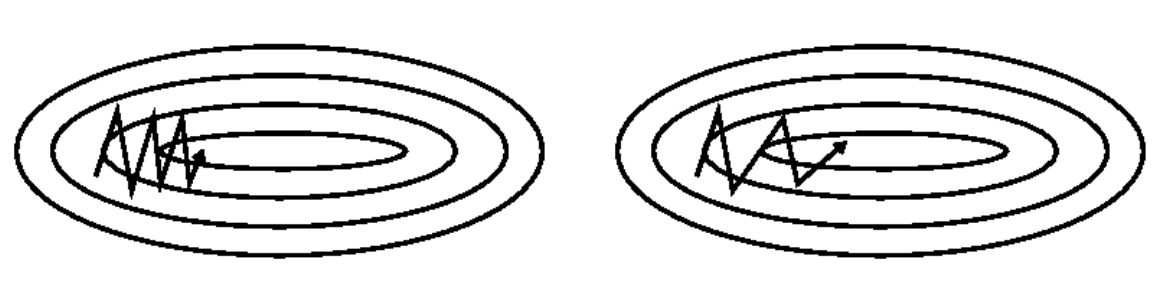
\includegraphics[width=0.5\linewidth]{images/smd/momentum.PNG}
    \caption{Left — SGD without momentum, right— SGD with momentum.}
    \label{fig:smd_momentum}
\end{figure}
\fi

\noindent The standard momentum descent is a technique first presented by Polyak \cite{POLYAK19641} that introduces a variable $V$ which accumulates the velocity towards directions of persisted reduction in the objective across iterates \cite{pmlr-v28-sutskever13}. The momentum algorithm allows to accelerate the gradient descent as in the detected direction it adds a fraction $\beta$ of the vector calculated in the previous step to the current update vector. The hyper-parameters are the learning rate $\eta$ and the momentum $\beta \in [0,1)$, the latter typically chosen as 0.9. If $\beta = 0$, then classical momentum reduces to the gradient method. The parameters update works as follow: 
\begin{subequations}
    \begin{equation}
        V_{dw} = \beta V_{dw} - \eta*dW
    \end{equation}
    \begin{equation}
        W = W + V_{dw}
    \end{equation}
    \label{eq:momentum_descent}
\end{subequations}

\subsection{Solving LLS with standard momentum descent}
The idea behind gradient descent is pretty similar to the one seen for conjugate gradient. Gradient descent can be used to solve a system of linear equation $Ax - b = 0$, where $A$ is symmetric and positive definite, but, as we know, the $\hat{X}$ matrix has not the same proprieties of $A$, so in order to apply gradient descent to our problem we need to define $A = \hat{X}^T \hat{X}$ and $b = \hat{X}^T \hat{y}$. We have already explained this fact when we described how to solve LLS problem while using conjugate gradient in \ref{subsec:solve_LLS_cg}. For this reason, we will not talk again about the preliminary part to do before starting to apply the algorithm.
\vspace{3mm}

\noindent The gradient descent algorithm differs a bit from the conjugate gradient one, so we are going to report it. Also, even for this algorithm, we do not explicitly compute the matrix $A$, even if it would have saved us time, because we preferred to get more qualitative results by limiting the condition number of $A$.

\begin{algorithm}[H]
    \caption{Standard momentum descent}
    \label{algorithm:smd_lls}
    Given $w_0 \in R^m$, $\beta$, $v = 0$;\\
    \While{$k<max\_iterations$ and $error \geq tol$} {
        $r_k=b-Aw_k$;\\
        $\eta = \frac{r_{k}^{T} r_{k}}{r_{k}^{T} A r_{k}}$;\\
        $v = \beta v + \eta r_k$;\\
        $w_k = w_k + v$;\\
        $k=k+1$;\\
    }
    \Return{$w$};
\end{algorithm}

\noindent The computational cost of gradient descent is dominated by matrix-vector products and fortunately, one can be eliminated. If we do not consider the momentum update rule, we get $w = w + \eta r_k$ and by premultiplying both sides of this equation by $-A$ and adding b, we have that
\begin{equation}
    r_k = r_k - \eta A r_k
    \label{eq:smd_rk}
\end{equation}
so we can store the result of $A r_k$ in order to avoid to compute it twice per iteration. The starting point for $r$ still remains $r_0 = b - A w_0$, then it gets updated by using the new formula. The disadvantage of using this recurrence is that the sequence defined by \eqref{eq:smd_rk} is generated without any feedback from the value of $w_i$, so that accumulation of floating point round-off error may cause $w_i$ to converge to some point near $w$. This effect can be avoided by periodically using $r_k=b-Aw_k$ to recompute the correct residual as suggested by Shewchuk et al. \cite{shewchuk1994introduction}.

\subsection{Convergence analysis with exact line search}\label{subsec:smd_convergence}
Assume that $f$ is strongly convex on $S$, so there are positive constants $\theta_1$ and $\theta_n$ such that $\theta_1I \leq \nabla^{2}f(x) \leq \theta_nI, \forall x \in S$. By using the lighter notation $x^{(k+1)} = x^{(k)} + \eta^{(k)}\Delta x^{(k)}$, Boyd and Vandenberghe \cite{boyd2004convex} state that
\begin{equation}
    f(x^{(k)}) - p^{*} \leq c^{k}(f(x^{(0)}) - p^{*})
    \label{eq:conv_grad_descent}
\end{equation}
where $p^*$ is the optimal value of the function $f$ and $c = 1 - \theta_1/\theta_n < 1$ \footnote{recalling that $\kappa = \theta_n/\theta_1 $ is an upper bound on the condition number of the matrix $\nabla^2f(x)$, \textit{i.e.} the ratio of its largest eigenvalue to its smallest eigenvalue.}, which shows that $f(x^{(k)})$ converges to $p^*$ as $k \rightarrow \infty$. In particular, we must have $f(x^{(k)}) - p^* \leq \epsilon$ after at most 
\begin{equation}
    \frac{log((f(x^{(0)})-p^*)/\epsilon)}{log(1/c)}
    \label{eq:iter_grad_descent}
\end{equation}
iterations of the gradient method with exact line search. We can now analyze what kind of information can be derived from both the numerator and the denominator. The first one can be interpreted as the log of the ratio of the initial sub-optimality (\textit{i.e.}, gap between $f(x^{0})$ and $p^*$, to the final sub-optimality (\textit{i.e.} less than $\epsilon$). This term
suggests that the number of iterations depends on how good the initial point is, and what the final required accuracy is. Instead, the denominator of \eqref{eq:iter_grad_descent} is a function of $\theta_n/\theta_1$, which we have seen is a bound on the condition number of $\nabla^2 f(x)$ and for large condition number bound $\theta_n/\theta_1$, we have 
\begin{equation}
    log(1/c) = -log(1-\theta_1/\theta_n) \approx \theta_1/\theta_n
\end{equation}
meaning that our bound on the number of iterations required increases approximately linearly following the increasing of $\theta_n/\theta_1$. This fact lead the gradient method to require a large number of iterations when the Hessian of $f$, near $x^*$, has a large condition number. Finally, the bound \eqref{eq:conv_grad_descent} shows that the error $f(x^{(k)}) - p^{*}$ converges to zero at least as fast as a geometric series that, in the context of iterative numerical methods, is called linear convergence.

\subsection{Convergence analysis of heavy ball}
\label{subsec:hbm_convergence}
Again, we know that $f$ is strongly convex on $S$, so there are positive constants $\theta_1$ and $\theta_n$ such that $\theta_1I \leq \nabla^{2}f(x) \leq \theta_nI, \forall x \in S$. The heavy ball method adds a momentum term in gradient descent:
\begin{equation}
    x_{k+1} = x_{k} - \eta_{k} \nabla_{x} f(x_k) + \underbrace{\beta_k (x_k - x_{k-1})}_{\text{HBM  momentum}}
    \label{eq:hb_update_xk}
\end{equation}

\noindent Consider $x_{k+1} - x^*$. By definition of HBM update \eqref{eq:hb_update_xk}, 
\begin{equation}
    x_{k+1} - x^* = x_{k} - \eta_{k} \nabla_{x} f(x_k) + \beta_k (x_k - x_{k-1}) - x^*
    \label{eq:hb_update_xk_2}
\end{equation}

\noindent As $\nabla_x f(x_k) = Ax_k - b$ and $b = Ax^*$, we have $\nabla_x f(x_k) = Ax_k - Ax^*$. By developing \eqref{eq:hb_update_xk_2}, we have:
\begin{equation}
\begin{aligned}
x_{k+1} - x^* &= x_k - x^* - \eta_k A(x_k - x^*) + \beta(x_k - x_{k-1}) \\
& = (I - \eta_k A)(x_k - x^*) + \beta_k (x_k - x_{k-1} -x^* + x^*) \\
& = (I - \eta_k A)(x_k - x^*) - \beta_k (x_{k-1} - x^*) + \beta(x_k - x^*)\\
&= \left((1+\beta_k)I-\eta_k A)\right(x_k - x^*) - \beta_k (x_{k-1} - x^*)
\end{aligned}
\end{equation}

\noindent In this sense, we have to consider $x_k - x^*$ and $x_{k-1} - x^* $ at the same time
\begin{equation}
\begin{bmatrix}
x_{k+1} - x^*\\
x_k - x^*
\end{bmatrix} 
=
\underbrace{\begin{bmatrix}
(1+\beta_k)I - \eta_k A & - \beta_kI\\
I & 0
\end{bmatrix}}_{T_k (\eta, \beta)}
\begin{bmatrix}
x_{k} - x^*\\
x_{k-1} - x^*
\end{bmatrix}
\end{equation}
where $T_k (\eta, \beta)$ is the transition matrix. For simplicity we consider the compact expression

\begin{equation}
\begin{bmatrix}
x_{k+1} - x^*\\
x_k - x^*
\end{bmatrix} 
=
T_k(\eta, \beta)
\begin{bmatrix}
x_{k} - x^*\\
x_{k-1} - x^*
\end{bmatrix}
\end{equation}
Take constant $\eta_k$ and $\beta_k$ in $T_k$, so $T_k = T$ and 

\begin{equation}
\begin{bmatrix}
x_{k+1} - x^*\\
x_k - x^*
\end{bmatrix} 
=
T^k
\begin{bmatrix}
x_{1} - x^*\\
x_{0} - x^*
\end{bmatrix}
\end{equation}
Take the norm

\begin{equation}
\left\lVert
\begin{bmatrix}
x_{k+1} - x^*\\
x_k - x^*
\end{bmatrix}
\right\rVert
=
\left\lVert
T^k
\begin{bmatrix}
x_{1} - x^*\\
x_{0} - x^*
\end{bmatrix}
\right\rVert
\leq
\lVert
T^k
\rVert
\left\lVert
\begin{bmatrix}
x_{1} - x^*\\
x_{0} - x^*
\end{bmatrix}
\right\rVert
\end{equation}
So, if $\lVert T^k \rVert$ is bounded, the series $x_k$ produced by the heavy ball method converges. In order to explain this we need two lemmas, for which we omit the proof.

\begin{lemma}
For a matrix $T \in \mathbb{R}^{n\times n}$, there exists a sequences $\epsilon_k \geq 0$ such that $\lVert T^k \rVert \leq (\rho(T) + \epsilon_k)^k$ where $\displaystyle \lim_{k \rightarrow \infty}{\epsilon_k = 0} $.
\label[lemma]{le:lemma1}
\end{lemma}

\begin{lemma}
For $\beta>(1 - \sqrt{\eta \theta_n})^2$, $\rho(T) < \beta$, where $\rho(T) = \max{\{|\psi_1|, |\psi_2|, \dots, |\psi_n|\}}$ is the spectral radius of matrix $T$ and $\psi_i$ are the eigenvalues of $T$.
%\label{le:lemma2}
\label[lemma]{le:lemma2}
\end{lemma}

\noindent Now, assume $\beta>(1 - \sqrt{\eta \theta_n})$, by \cref{le:lemma2} we have $\rho(T) = \max{|\psi_i(T)|} \leq \beta$. By \cref{le:lemma1}, we have $\lVert T^k \rVert \leq (\rho(T) + \epsilon_k)^k$ with $\displaystyle \lim_{k \rightarrow \infty}{\epsilon_k = 0}$. Putting \cref{le:lemma2} into \cref{le:lemma1} we obtain:
\begin{equation}
    \lVert T^k \rVert \leq (\beta + \epsilon_k)^k
\end{equation}

\vspace{3mm}

\noindent Lastly, let $\eta = \frac{4}{(\sqrt{\theta_n}+\sqrt{\theta_1})^2}$ and $\beta = \frac{\sqrt{\theta_n} - \sqrt{\theta_1}}{\sqrt{\theta_n}+\sqrt{\theta_1}}$ in $T$ we have:
\begin{equation}
\left\lVert
\begin{bmatrix}
x_{k+1} - x^*\\
x_k - x^*
\end{bmatrix}
\right \rVert
\leq \left(\frac{\sqrt{\theta_n} - \sqrt{\theta_1}}{\sqrt{\theta_n}+\sqrt{\theta_1}} + \epsilon \right)^k
\left\lVert
\begin{bmatrix}
x_{1} - x^*\\
x_{0} - x^*
\end{bmatrix}
\right\rVert
\end{equation}
or:
\begin{equation}
    \lVert x_k - x^* \rVert \leq \left(\frac{\sqrt{\kappa} - 1}{\sqrt{\kappa}+1} + \epsilon \right)^k \lVert x_0 - x^* \rVert
\end{equation}
 where $\kappa = \frac{\theta_n}{\theta_1}$. By exploiting momentum, we benefit of an improvement from $ \left(\frac{\kappa - 1}{\kappa + 1} + \epsilon \right)^k$ of the standard gradient descent to $\left(\frac{\sqrt{\kappa} - 1}{\sqrt{\kappa}+1} + \epsilon \right)^k$ of the heavy ball method. This result is similar to the one obtained for the conjugate gradient method, in \eqref{eq:cg_rewritten_epsilon}.

\subsection{Performance analysis}

\subsubsection{Linear rate of convergence}
In \ref{subsec:hbm_convergence}, we stated that the standard momentum descent algorithm has a linear convergence rate due to the fact that our function is strongly convex.
\vspace{3mm}

\noindent In \autoref{fig:convergence_smd} we can empirically confirm that our implementation has the theoretically expected convergence rate. Moreover we can notice that when $\hat{X}^T\hat{X}$ becomes more and more ill-conditioned, the GD method requires more steps to converge, as discussed in \ref{subsec:smd_convergence}.

\begin{figure}[H]
    \centering
    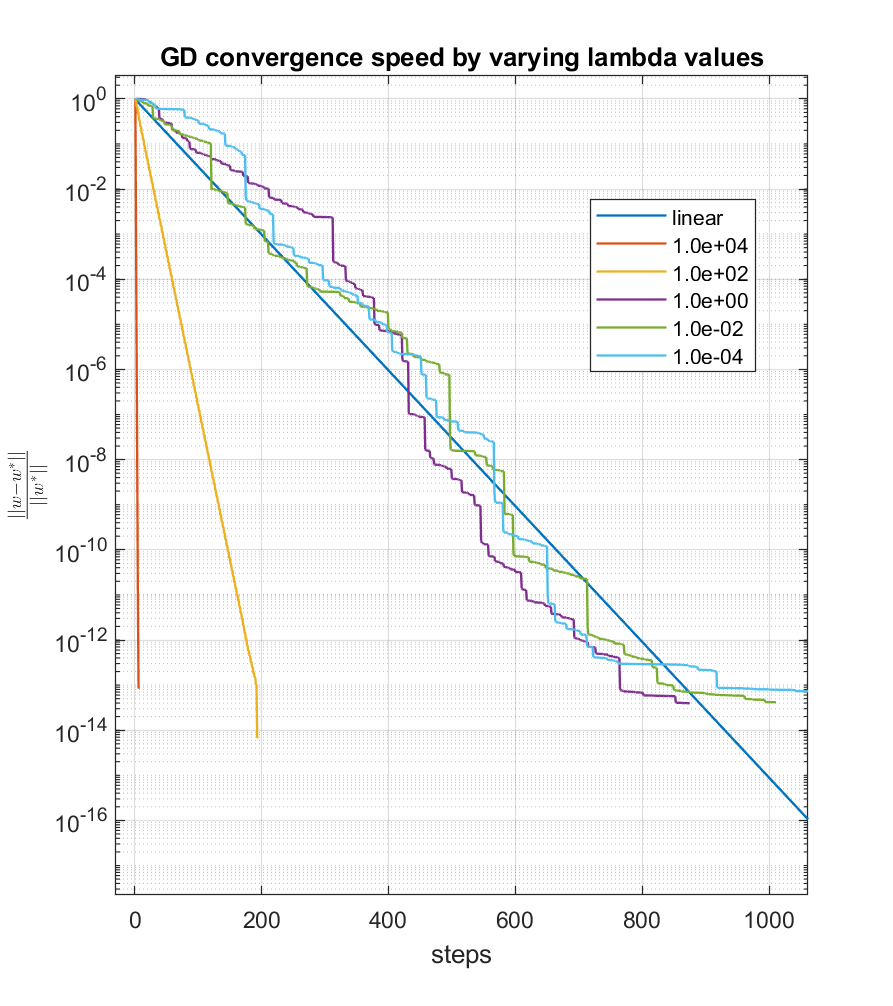
\includegraphics[width = 0.7\linewidth]{images/smd/momentum_comparison_smd_linear_fixed.png}
    \caption{GD convergence speed by varying lambdas values, with momentum.}
    \label{fig:convergence_smd}
\end{figure}

\subsubsection{Effect of momentum}
A fundamental analysis involves the role of $\beta$ in our method, therefore,
in order to find the best value for such hyper-parameter, we ran a grid search. For instance, in \autoref{fig:smd_comparing_betas}, we fixed the problem (same input matrix, expected values and starting point) and we found that the best value for $\beta$ was equal to $0.05$, of course, this value can greatly differ from problem to problem. In our case, a too high momentum slows down the convergence speed, increasing the total amount of steps needed to reach the convergence.

\begin{figure}[H]
    \centering
    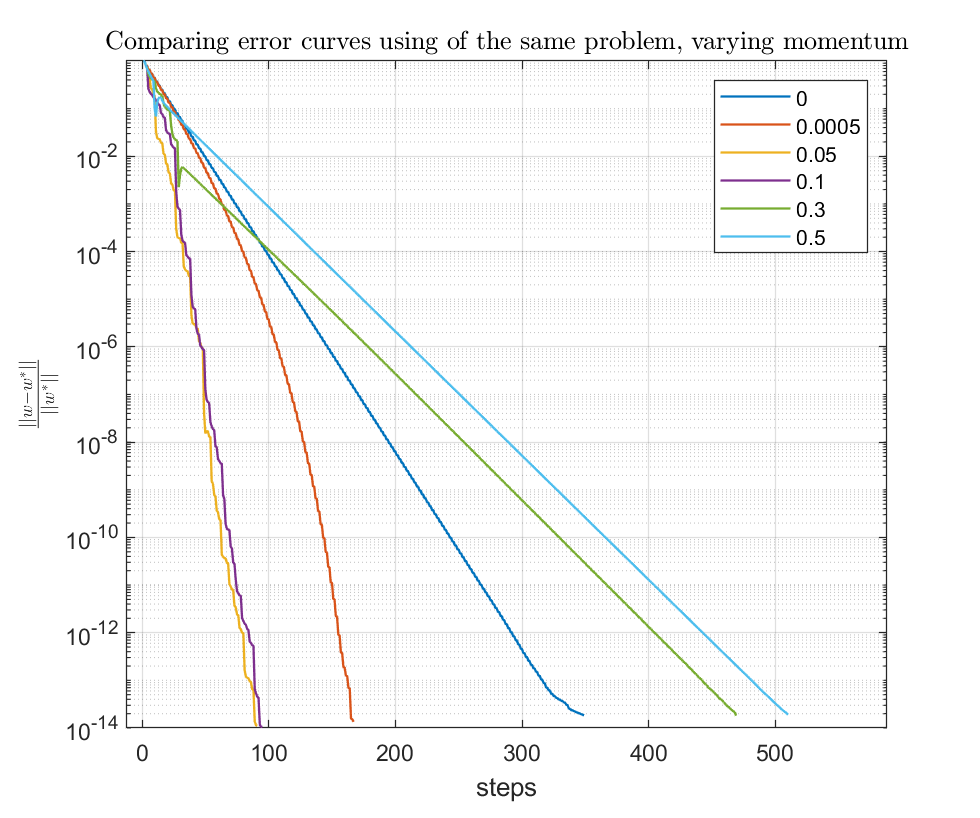
\includegraphics[width = 0.8\linewidth]{images/smd/momentum_comparison_smd.png}
    \caption{GD convergence speed by varying $\beta$ values.}
    \label{fig:smd_comparing_betas}
\end{figure}

\noindent It is interesting to notice that the introduction of momentum makes our method faster, when chosen appropriately, but, on the other side, we can say that it becomes more unstable by looking at \autoref{fig:smd_comparing_betas}.

\paragraph{Side by side comparison}
We will now graphically view the effect of momentum in reducing the total amount of steps required by the gradient descent to converge. In \autoref{fig:smd_with_without_momentum} it is clearly visible that momentum plays an important role, in fact it allowed us to reduce the total amount of steps to reach the convergence especially when the Hessian becomes ill-conditioned.

\begin{figure}[H]
    \centering
    \subfloat[Gradient descent with momentum]{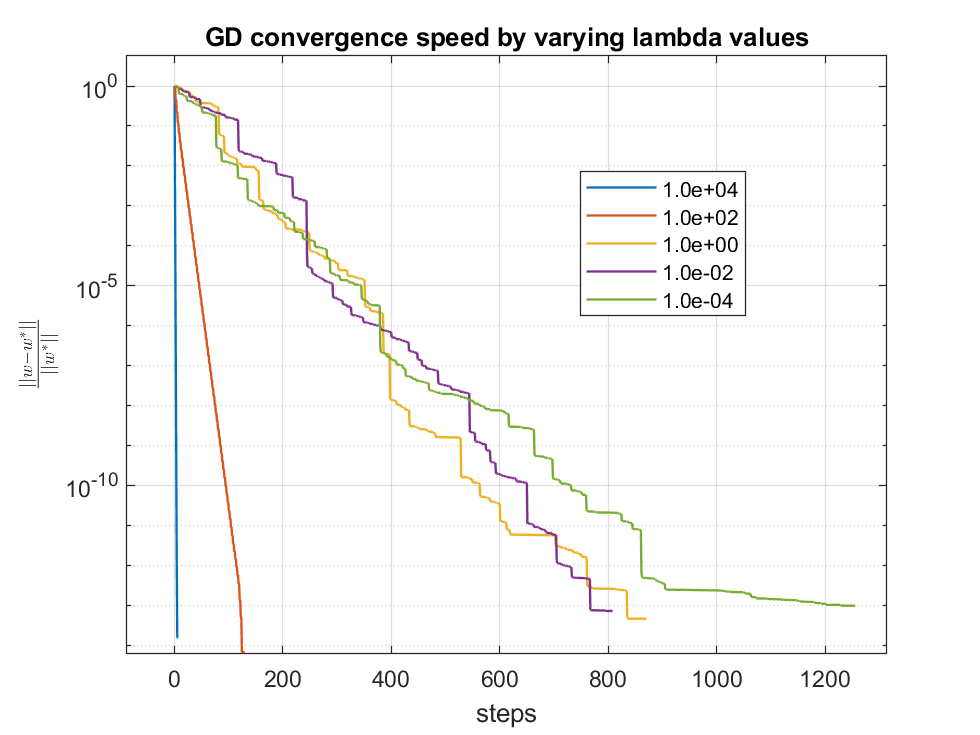
\includegraphics[width=0.52\linewidth]{images/smd/smd_comparison_with_momentum.png}}
    \subfloat[Gradient descent without applying momentum]{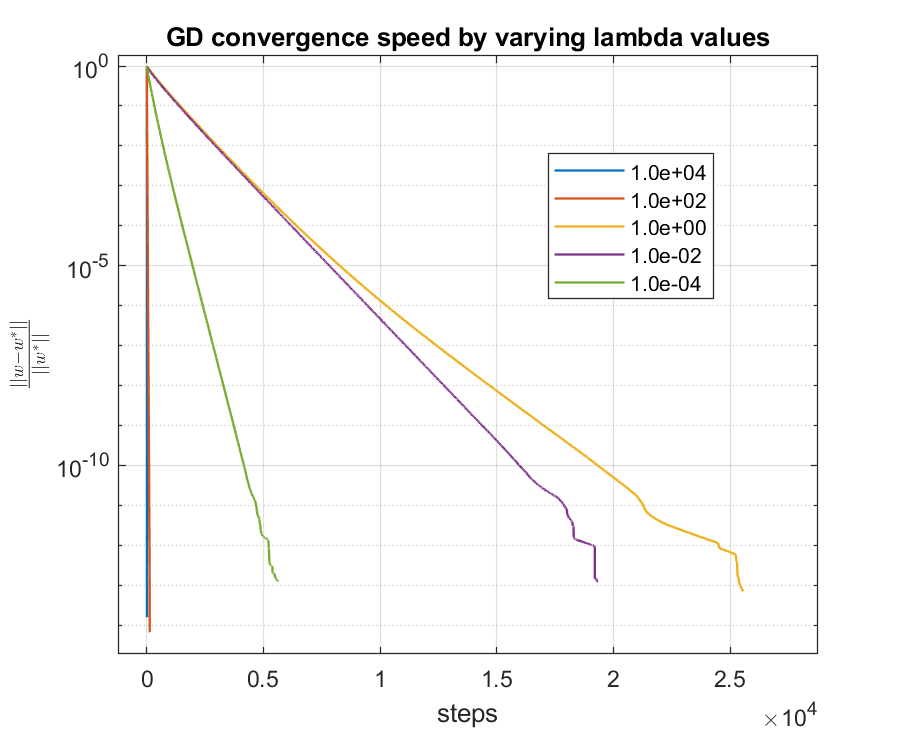
\includegraphics[width=0.48\linewidth]{images/smd/smd_comparison_no_momentum.png}}
    \caption{Side by side comparison between the steps necessary to converge by GD method, with and without momentum.}
    \label{fig:smd_with_without_momentum}
\end{figure}

\subsubsection{Results}
By looking at \autoref{tab:smd_results}, it is possible to notice that the relative errors and the relative residuals are pretty similar to the conjugate gradient ones from \autoref{tab:cg_results}, since the two methods are related. Furthermore, in terms of relative error and amount of steps to reach the convergence, the algorithm performed better without using momentum only for $\lambda = 10^4$, whereas, in the remaining cases we tested, adding momentum allowed us to reach the solution in a faster way as already seen from \autoref{fig:smd_with_without_momentum}. As usual, $w^*$ is the Matlab solution $\hat{X}\backslash \hat{y}$ and, from \ref{subsec:introduction_convexity}, such minima is unique and global.

\begin{table}[H]
\small
\centering
\begin{tabular}{c|c|c|c|c|c} \hline \hline
    $\lambda$& $\beta$ &$\frac{\lVert w - w^{*} \lVert}{\rVert w^{*} \lVert}$ & $\frac{\lVert \hat{X}w - y \lVert }{\lVert y \lVert}$ & steps & time (sec)\\ \hline \hline
    
    \rowcolor{gray!30} $10^4$ & $0$ & $ 3.49 \times 10^{-14} \pm 2.15 \times 10^{-14}$ &$9.99 \times 10^{-1} \pm 3.04 \times 10^{-4}$ & $19 \pm 9$& $9.56 \times 10^{-4}$ \\
    
    $10^2$ & $ 0.05$ & $ 8.67 \times 10^{-15} \pm 8.08 \times 10^{-16}$ &$9.39 \times 10^{-1} \pm 4.21 \times 10^{-2}$&$106 \pm 10$& $4.12 \times 10^{-3}$ \\
    
    \rowcolor{gray!30} $1$ & $0.05$ & $ 3.51 \times 10^{-14} \pm 1.85 \times 10^{-14} $ &$ 5.61 \times 10^{-2} \pm 5.66 \times 10^{-3} $&$1350 \pm 342$& $4.91 \times 10^{-2}$ \\
    
    $10^{-2}$ & $ 0.05$ & $5.77 \times 10^{-14} \pm 3.08 \times 10^{-14}$ & $5.07 \times 10^{-4} \pm 7.58 \times 10^{-5}$&$1075 \pm 78$& $3.84 \times 10^{-2}$ \\
    
    \rowcolor{gray!30} $10^{-4}$ & $0.05$ & $6.42 \times 10^{-14} \pm 2.57 \times 10^{-14}$ &$5.42 \times 10^{-6} \pm 8.26 \times 10^{-7}$&$1148 \pm 59$ & $4.10 \times 10^{-2}$ \\
    \hline \hline
\end{tabular}
\caption{Standard momentum descent results.}
\label{tab:smd_results}
\end{table}

\section{Comparison between methods}
As last step for this report we will blend together all the results achieved by the four different methods illustrated by, first, comparing the three iterative methods on time metrics and, then, by comparing all of them based on errors and residuals. Keep in mind that the results shown here and in all the tables before were achieved with starting point $x_0=0$, since we have empirically seen it to be the best choice.

\subsection{Comparison on time metrics}
We will start by considering only three of the methods seen until now (L-BFGS, CG and SMD) since thin QR is not iterative. \autoref{tab:time_comparison} shows the execution times and number of iterations achieved by the best configuration of these three methods:
\begin{itemize}
    \item For the L-BFGS method the best results were retrieved from \autoref{tab:lbfgs_results} where $l=20$.
    \item Conjugate gradient had no hyper-parameters, so the results are those seen from \autoref{tab:cg_results}.
    \item For standard momentum descent the results are those from \autoref{tab:smd_results}, following the grid search for the best values of $\beta$.
\end{itemize}

\begin{table}[H]
\centering
\begin{tabular}{c|c|c|c|c|c|c} \hline \hline
    \multirow{2}{*}{$\lambda$} & \multicolumn{2}{c|}{L-BFGS} & \multicolumn{2}{c|}{CG} & \multicolumn{2}{c}{SMD} \\ \cline{2-7}
    & time & steps & time & steps & time & steps \\ \hline \hline
    
    \rowcolor{gray!30} $10^4$ & $3.0\times10^{-3}$ & $4$ & $5.5\times 10^{-4}$ & $4$ & $9.5 \times 10^{-4}$ & 19 \\
    
    $10^2$ & $3.5\times10^{-3}$ & $10$ & $1.2\times 10^{-3}$ & $10$ & $4.1 \times 10^{-3}$ & 106 \\
    
    \rowcolor{gray!30} $1$ & $3.8\times10^{-3}$ & $13$ & $1.8\times 10^{-3}$ & $18$ & $4.9 \times 10^{-2}$ & $1350$ \\
    
    $10^{-2}$ & $3.9\times10^{-3}$ & $13$ & $1.9\times 10^{-3}$ & 17 & $3.8 \times 10^{-2}$ & $1075$ \\
    
    \rowcolor{gray!30} $10^{-4}$ & $4.0\times10^{-3}$ & $13$ & $2.0\times 10^{-3}$ & $18$ & $4.1 \times 10^{-2}$ & $1148$ \\
    \hline \hline
\end{tabular}
\caption{Comparison on execution time (in seconds) and number of iterations between the three iterative methods.}
\label{tab:time_comparison}
\end{table}

\noindent As we can see from \autoref{tab:time_comparison} L-BFGS and conjugate gradient methods performs in a similar way, instead SMD has an higher number of iterations and execution time as $\lambda$ starts to get smaller and smaller, this is expected since standard momentum descent is just a poorer version of conjugate gradient.
\vspace{3mm}

\noindent Between L-BFGS and conjugate gradient, the former has a low number of iteration but double the execution time, so, at the end, the best iterative algorithm, in our case, would be conjugate gradient.

\subsection{Comparison on metrics}
Let us now talk about the comparison on errors and residuals, this time including the results achieved by the thin QR factorization. The results are shown in \autoref{tab:errors_comparison}.
\begin{table}[H]
\centering
\begin{tabular}{c|c|c|c|c}
    \hline \hline
    \multirow{2}{*}{$\lambda$} & \multicolumn{2}{c|}{L-BFGS} & \multicolumn{2}{c}{Thin QR} \\ \cline{2-5}
    & error & residual & error & residual \\ \hline \hline
    
    \rowcolor{gray!30} $10^4$ & $1.40 \times 10^{-14}$ &$9.99 \times 10^{-1}$& $7.38 \times 10^{-14}$ & $9.99 \times 10^{-1}$  \\
    
    $10^2$ & $5.62 \times 10^{-15}$ & $9.37 \times 10^{-1}$ & $1.56\times 10^{-14}$ & $9.11 \times 10^{-1}$ \\
    
    \rowcolor{gray!30} $1$ & $1.73 \times 10^{-14}$ &$5.89 \times 10^{-2}$ & $2.03 \times 10^{-14}$ & $5.34 \times 10^{-2}$ \\
    
    $10^{-2}$ & $2.72 \times 10^{-14}$ & $5.02 \times 10^{-4}$ & $9.01 \times 10^{-14}$ & $5.44 \times 10^{-4}$ \\
    
    \rowcolor{gray!30} $10^{-4}$& $4.07 \times 10^{-14}$& $6.08 \times 10^{-6}$ & $8.17 \times 10^{-14}$ & $5.40 \times 10^{-6}$\\
    \hline
    
    \end{tabular} \\
    \begin{tabular}{c|c|c|c|c}
    \hline
    \multirow{2}{*}{$\lambda$} & \multicolumn{2}{c|}{CG} & \multicolumn{2}{c}{SMD} \\ \cline{2-5}
    & error & residual & error & residual \\ \hline \hline
    
    \rowcolor{gray!30} $10^4$ & $2.76 \times 10^{-14}$ & $ 9.99 \times 10^{-1}$& $3.49 \times 10^{-14}$ & $9.99 \times 10^{-1}$  \\
    
    $10^2$ & $ 1.47 \times 10^{-14}$ & $ 9.33 \times 10^{-1}$ & $8.67\times 10^{-14}$ & $9.39 \times 10^{-1}$ \\
    
    \rowcolor{gray!30} $1$ & $2.03\times 10^{-14}$ & $ 5.60 \times 10^{-2}$ & $3.51 \times 10^{-14}$ & $5.61 \times 10^{-2}$ \\
    
    $10^{-2}$ & $2.75 \times 10^{-14} $ & $5.54 \times 10^{-4}$ & $5.77 \times 10^{-14}$ & $5.07 \times 10^{-4}$ \\
    
    \rowcolor{gray!30} $10^{-4}$& $2.79 \times 10^{-14}$ & $5.22 \times 10^{-6}$ & $6.42 \times 10^{-14}$ & $5.42 \times 10^{-6}$\\
    \hline \hline
    
    \end{tabular}
\caption{Comparison on relative errors and residuals.}
\label{tab:errors_comparison}
\end{table}

\noindent By analyzing the errors and residuals obtained by the algorithms, we notice that they are pretty similar, and this is maybe due to the fact that our function is strongly convex, therefore, it was quite easy to find the unique global minimum and, as a consequence, we had the nice possibility to use the exact line search for those algorithm that required a line search. As we can see in \autoref{tab:errors_comparison}, in terms of relative errors, L-BFGS performs better with respect to the others, but not significantly noticing that the order of magnitude is the same of the other algorithms.
\vspace{3mm}

\noindent Another aspect to consider is that the performances of SMD and L-BFGS depend on their hyper-parameters. We are referring to the memory size $l$ for L-BFGS and to the step size $\eta$ and the momentum $\beta$ for SMD. The first hyper-parameter of the latter is useful only for the fixed step length version, that often requires a grid search before being chosen, as well as for the momentum. To clarify, the choice of a too low memory size of L-BFGS could slow down the convergence rate, but eventually the algorithm finds a solution, instead this does not happen if the learning rate is chosen wrongly, since it could cause the SMD to diverge. Rather, thin QR and conjugate gradient are ready-to-use algorithms that do not require hyper-parameters tuning, so they are easier to set up.

\subsection{Comparison on space}
Now, we can analyze these algorithms in terms of space complexity. Starting with thin QR, we notice that is the one using more memory because it stores the upper triangular matrix $R_1$ and the vector resulting from the product $Q_1 \hat{y}$, because we do not explicitly compute $Q_1$.
\vspace{3mm}

\noindent Then, we have conjugate gradient and standard momentum descent that are the lightest, in fact they only need few arrays: both require one for the solution, and one for the residual $r_k$ whereas CG needs one more for $p_k$ and SMD needs another one for the $v$ array in order to update the solution. In the end we have L-BFGS, whose space complexity is dominated by the two matrices $S,Y \in \mathbb{R}^{n\times l}$, where $n$ is the size of the solution and $l$ is the memory size, plus the same space required by the last two aforementioned algorithms. Let us say that L-BFGS uses less memory than thin QR when $l < \frac{n}{2}$, which always holds for our case since $n=1477$ and $l \in [3, 20]$.

\subsection{Comparison on scalability}
As final comparison we will compare the scalability of each method in a similar fashion to what we have done in \ref{subsec:qr_linearity}. We generated $20$ matrices and we run each every method five times on them, then we averaged the results in order to compare the methods' behavior as the size of the problem increases. As first test we fixed the number of columns to $200$ and we let the number of rows grow by $250$ at every new generated matrix, starting from $1000$. Afterwards, for the second test, we performed the same task of the first one but, this time, we also increased the number of columns by $50$ at each step to see how the methods scale when both sizes increase.
\begin{figure}[H]
    \centering
    \subfloat[Scalability by varying the number of rows \label{subfig:scalability_rows}]{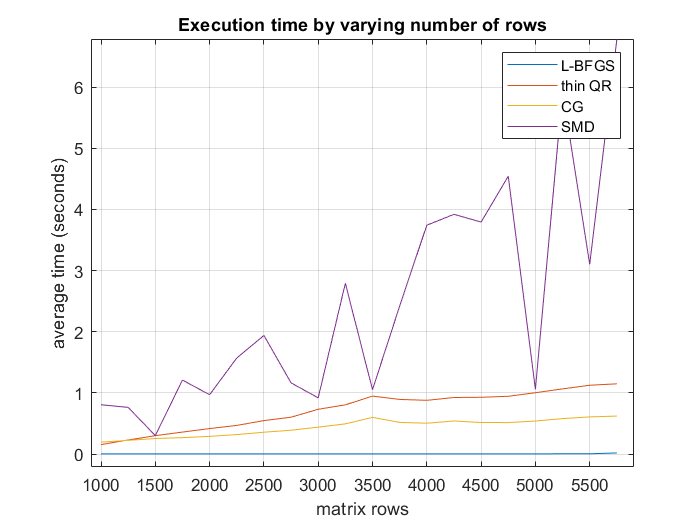
\includegraphics[width=0.5\linewidth]{images/comparisons/comparison_scalabiltiy_rows.png}}
    \subfloat[Scalabilty by varying both sizes \label{subfig:scalability}]{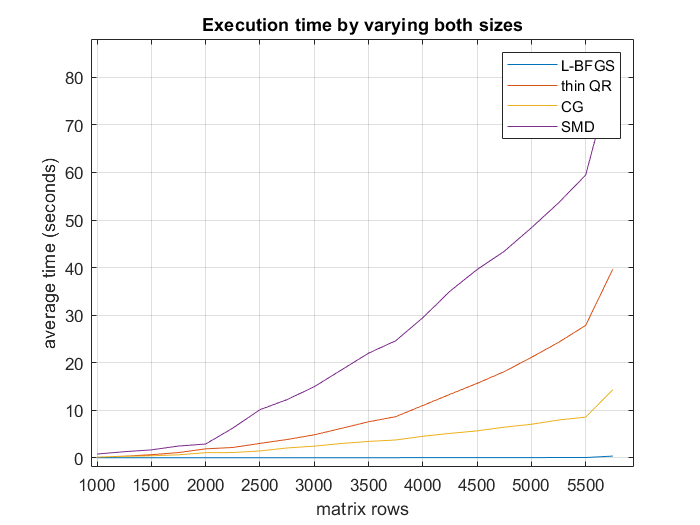
\includegraphics[width=0.5\linewidth]{images/comparisons/comparison_scalability.png}}
    \caption{Scalability comparison between the four methods, first by only varying the number of rows and then by varying both sizes.}
    \label{fig:comparison_scalability}
\end{figure}

\noindent As we can see from \autoref{fig:comparison_scalability} standard momentum descent performs worse than the other three methods since we could not do an exhaustive grid search to look for the best value of $\beta$ for each configuration. Other than that, from both figures we can notice that L-BFGS (with $l=20$) is the uncontested winner since it suffers a little from the increase in size of the matrix. Moreover, by looking at \autoref{subfig:scalability} we can see that thin QR is the one suffering the most by the increase in columns, as expected from the theory, meanwhile the others maintain, more or less, the same behavior, except for SMD which seems more stable than what we can see in \autoref{subfig:scalability_rows} at the cost of an even worse scalability.

\section{How to run the project}\label{sec:how_to_run_project}
First, you can clone the project repo from github in the following way
\begin{minted}[fontsize=\small, breaklines]{bash}
git clone https://github.com/nikodallanoce/ComputationalMathematics/
\end{minted}
Then you can work with each method separately on Matlab by going inside the chosen algorithm folder and running \textit{run\_method.m}, change the hyper-parameters as you prefer.

\appendix
\section{Appendix of proofs}
\subsection{\texorpdfstring{$\lambda$}{{}} is the smallest singular value of \texorpdfstring{$\hat{X}$}{{}}}\label{appendix:smallest_singular_value}
\noindent For that we need to follow what \cite{THOMPSON19721} has stated in theorem 1 and apply it to our case, therefore: let $\hat{X}$ be an $m\times n$ matrix where $\hat{X}=\begin{bmatrix}
    X^T\\
    \lambda I
\end{bmatrix}$ with $X^T \in \mathbb{R}^{k\times n}$, whose singular values are $\sigma_1(\hat{X})\geq \dots \geq \sigma_n(\hat{X})$. Let $\lambda I$ be a $n\times n$ submatrix of $\hat{X}$, with singular values $\sigma_1(\lambda I)\geq \dots \geq \sigma_n(\lambda I)$, then
\begin{subequations}
    \begin{equation}
        \label{eq:proof_singular_value_1}
        \sigma_i(\hat{X}) \geq \sigma_i(\lambda I), \hspace{3mm }for \hspace{3mm} i=1,\dots, n
    \end{equation}
    \begin{equation}
        \label{eq:proof_singular_value_2}
        \sigma_i(\lambda I) \geq \sigma_{i+k}(\hat{X}), \hspace{3mm }for \hspace{3mm} i\leq min(n-k, n)
    \end{equation}
    with $k=m-n$.
\label{eq:proof_singular_value}
\end{subequations}
\vspace{3mm}

\noindent Let's consider the $(n-k)th$ singular value of $\lambda I$, following \eqref{eq:proof_singular_value_2} we have that
\begin{equation}
    \sigma_n(\hat{X}) \leq \sigma_{n-k}(\lambda I)
    \label{eq:proof_singular_value_3}
\end{equation}
Then by putting \eqref{eq:proof_singular_value_1} into \eqref{eq:proof_singular_value_3} we obtain
\begin{equation}
    \sigma_n(\lambda I) \leq \sigma_n(\hat{X}) \leq \sigma_{n-k}(\lambda I)
    \label{eq:proof_singular_value_4}
\end{equation}
$\lambda I$ is an $n\times n$ matrix whose singular values are all equal to $\lambda$, therefore from \eqref{eq:proof_singular_value_4} we can easily state that
\begin{equation}
    \sigma_n(\hat{X})=\lambda
    \label{eq:least_singular_value}
\end{equation}

\subsection{Condition number of \texorpdfstring{$\hat{X}$}{{}}}\label{appendix:condition_number}
As we know from the theory, the condition number $\kappa$ of a matrix is the following
\begin{equation}
    \kappa(\hat{X}) = \frac{\sigma_1}{\sigma_n}
    \label{eq:condition_number}
\end{equation}
where $\sigma_1$ and $\sigma_n$ are the biggest and smaller singular values of $\hat{X}$ and we already know from \ref{appendix:smallest_singular_value} that the latter is $\lambda$. Therefore, as $\lambda$ decreases the more $\kappa(\hat{X})$ increases, formally
\begin{equation}
    \lim_{\lambda \rightarrow 0} \kappa(\hat{X}) = \lim_{\lambda \rightarrow 0} \frac{\sigma_1}{\lambda} = \infty
    \label{eq:condition_number_formal}
\end{equation}
We will show, as last thing, that \eqref{eq:condition_number_formal} holds by looking at how $\kappa(\hat{X})$ changes at different values of $\lambda$ in \autoref{tab:condition_number}
\begin{table}[H]
\centering
\begin{tabular}{c|c}
    \hline \hline
    $\lambda$ & $\kappa(\hat{X})$ \\ \hline \hline
    $10^4$ & 1.0034 \\
    $10^2$ & 8.32 \\
    $1$ & 825.532 \\ 
    $10^{-2}$ & $8.255 \times 10^{4}$ \\
    $10^{-4}$ & $8.255 \times 10^{6}$ \\
    \hline
\end{tabular}
\caption{$K(\hat{X})$ at varying values of $\lambda$}
\label{tab:condition_number}
\end{table}

\subsection{Distinct eigenvalues of \texorpdfstring{$\hat{X}^T\hat{X}$}{{}}}\label{appendix:eigenvalues_singular_values}
We know from \ref{appendix:smallest_singular_value} that the submatrix $\lambda I \in \mathbb{R}^n$ has only one distinct singular value, that is $\lambda$. Moreover, the upper component of $\hat{X}$, $X^T$ has $m-n=12$ distinct singular values.
\vspace{3mm}

\noindent Now, since we know that 
\begin{equation}
    eig(\hat{X}^T \hat{X}) = \Sigma^2(\hat{X})
    \label{eq:appendix_sv}
\end{equation}

\noindent we can safely state that $\hat{X}^T\hat{X}$ has $m-n+1$ distinct eigenvalues, for the case under our consideration there are $13$ of them.

\newpage

\section{Appendix of plots}
\subsection{L-BFGS}\label{appendix:lbfgs_plots}
\begin{figure}[H]
    \centering
    \subfloat[Considering the convergence rates]{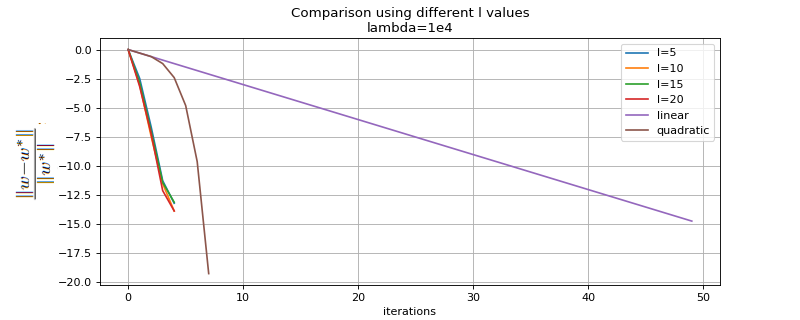
\includegraphics[width=0.8\linewidth]{images/lbfgs/lambda1e4.png}} \\
    \subfloat[Without the convergence rates]{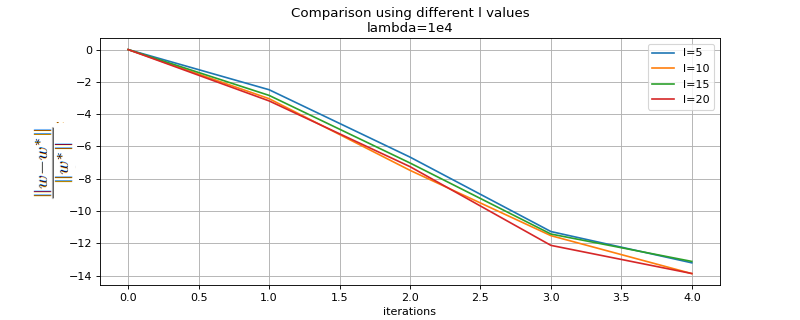
\includegraphics[width=0.8\linewidth]{images/lbfgs/lambda_wout_1e4.png}}
    \caption{Convergence plot with $\lambda=1e4$ at varying values of $l$}
    \label{fig:lbfgs_1e4_l}
\end{figure}

\begin{figure}[H]
    \centering
    \subfloat[Considering the convergence rates]{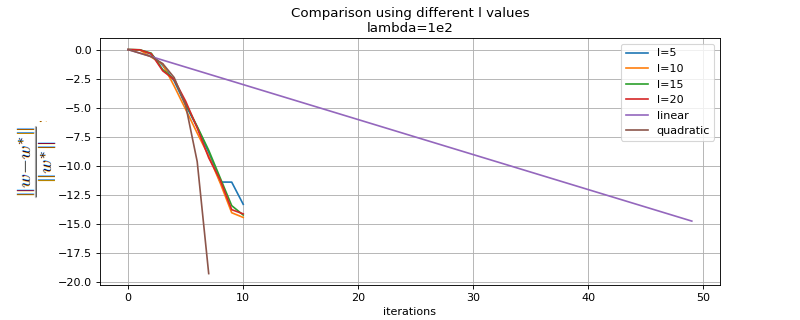
\includegraphics[width=0.8\linewidth]{images/lbfgs/lambda1e2.png}} \\
    \subfloat[Without the convergence rates]{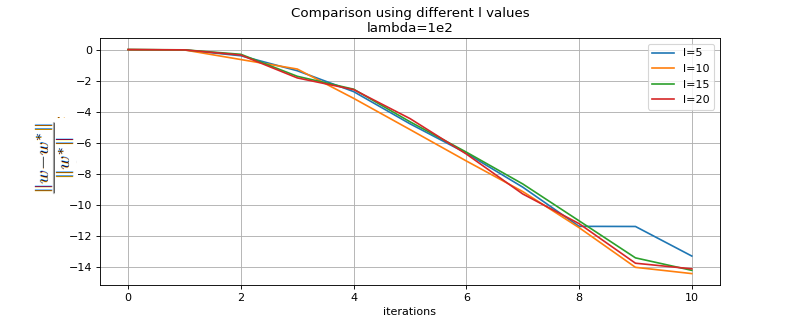
\includegraphics[width=0.8\linewidth]{images/lbfgs/lambda_wout_1e2.png}}
    \caption{Convergence plot with $\lambda=1e2$ at varying values of $l$}
    \label{fig:lbfgs_1e2_l}
\end{figure}


\begin{figure}[H]
    \centering
    \subfloat[Considering the convergence rates]{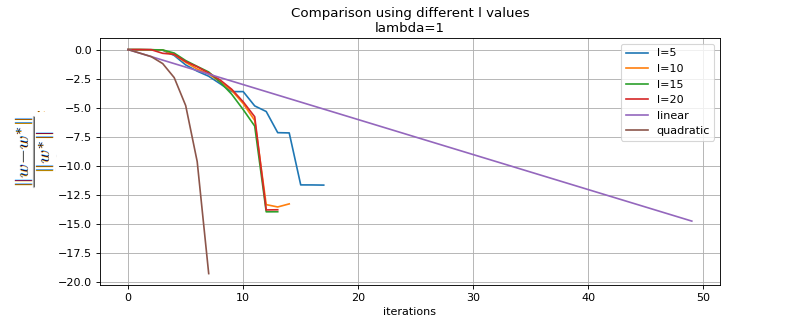
\includegraphics[width=0.8\linewidth]{images/lbfgs/lambda1.png}} \\
    \subfloat[Without the convergence rates]{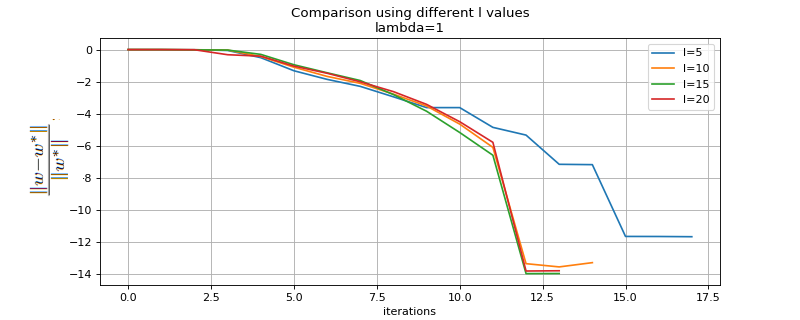
\includegraphics[width=0.8\linewidth]{images/lbfgs/lambda_wout_1.png}}
    \caption{Convergence plot with $\lambda=1$ at varying values of $l$}
    \label{fig:lbfgs_1_l}
\end{figure}

\begin{figure}[H]
    \centering
    \subfloat[Considering the convergence rates]{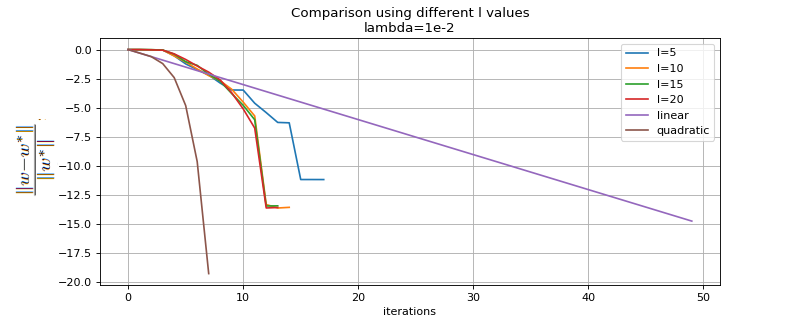
\includegraphics[width=0.8\linewidth]{images/lbfgs/lambda1e-2.png}} \\
    \subfloat[Without the convergence rates]{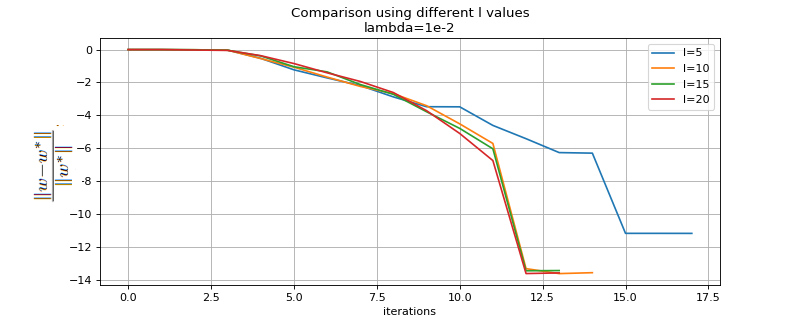
\includegraphics[width=0.8\linewidth]{images/lbfgs/lambda_wout_1e-2.png}}
    \caption{Convergence plot with $\lambda=1e-2$ at varying values of $l$}
    \label{fig:lbfgs_1e-2_l}
\end{figure}

\begin{figure}[H]
    \centering
    \subfloat[Considering the convergence rates]{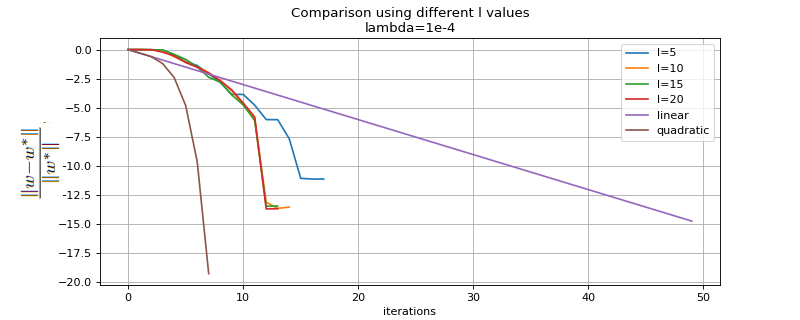
\includegraphics[width=0.8\linewidth]{images/lbfgs/lambda1e-4.png}} \\
    \subfloat[Without the convergence rates]{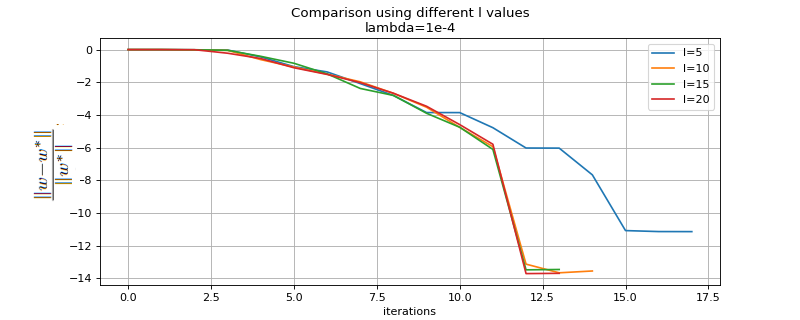
\includegraphics[width=0.8\linewidth]{images/lbfgs/lambda_wout_1e-4.png}}
    \caption{Convergence plot with $\lambda=1e-4$ at varying values of $l$}
    \label{fig:lbfgs_1e-4_l}
\end{figure}

\section*{References}
%From where you are taking information, where a reader can find details, credits, sources \dots See any paper bibliography to take examples. The items here should be numbered and the number should be used in the text. \textbf{Double check the bibliography}!!! \\ \\
%In particular, always include (with a uniform style): \\

%Authors, Title, Journal/Proceedings/Editor, Volume, Pages, Year (URL if needed) \\ %\\
%E.g.: 
%\bibliographystyle{plain}
\setcitestyle{square}
\bibliographystyle{plain}
\thispagestyle{empty}
\pagenumbering{gobble}
\vspace{-1cm}\bibliography{references}
\end{document}
